\documentclass[11pt,a4paper]{article}
\usepackage[utf8]{inputenc}
\usepackage[T1]{fontenc}
\usepackage[margin=2.5cm]{geometry}
\usepackage{authblk,amsmath,amssymb,booktabs,longtable,array,graphicx,placeins}
\usepackage[hidelinks]{hyperref}
\emergencystretch=3em
\renewcommand{\thesection}{S\arabic{section}}
\title{Supplementary information: a causal--ontological digital twin answers management questions for the world's largest sand desert}
\newcommand{\ReferenceMAGs}{5438}
\newcommand{\CBBFull}{232}
\newcommand{\HtwoCBB}{136}
\newcommand{\HtwoCBBStrict}{100}
\newcommand{\ArchaealRuBisCO}{241}
\newcommand{\DualHtwoCO}{34}
\newcommand{\HtwoCarriers}{1094}
\newcommand{\MultiHtwoMAGs}{47}
\newcommand{\JustAxioms}{38}
\newcommand{\AmbiguousSamples}{549}
\newcommand{\ForecastVisits}{409}
\newcommand{\TestVisits}{278}
\newcommand{\ConformalCoverage}{85.3\%}
\newcommand{\RankReversals}{1}

% Generated by reproducibility/v06/tables.py; do not edit by hand.
\newcommand{\MappedSamples}{550}
\newcommand{\ClosedCOGates}{8}
\newcommand{\ClosedHtwoGates}{0}
\newcommand{\ClosedCOZeroEffects}{48}
\newcommand{\ClosedCOAllZero}{yes}
\newcommand{\HtwoGateSingleMedianSurface}{1102.3}
\newcommand{\HtwoGateSingleQOneSurface}{1102.3}
\newcommand{\HtwoGateSingleQThreeSurface}{1102.3}
\newcommand{\HtwoGateSingleNSurface}{117}
\newcommand{\HtwoGateSingleMedianDeep}{1102.3}
\newcommand{\HtwoGateSingleQOneDeep}{1102.3}
\newcommand{\HtwoGateSingleQThreeDeep}{1102.3}
\newcommand{\HtwoGateSingleNDeep}{165}
\newcommand{\HtwoGateSingleMedianRoot}{1102.3}
\newcommand{\HtwoGateSingleQOneRoot}{1102.3}
\newcommand{\HtwoGateSingleQThreeRoot}{1102.3}
\newcommand{\HtwoGateSingleNRoot}{268}
\newcommand{\COGateSingleMedianSurface}{144.4}
\newcommand{\COGateSingleQOneSurface}{144.4}
\newcommand{\COGateSingleQThreeSurface}{144.4}
\newcommand{\COGateSingleNSurface}{117}
\newcommand{\COGateSingleMedianDeep}{144.4}
\newcommand{\COGateSingleQOneDeep}{144.4}
\newcommand{\COGateSingleQThreeDeep}{144.4}
\newcommand{\COGateSingleNDeep}{165}
\newcommand{\COGateSingleMedianRoot}{144.4}
\newcommand{\COGateSingleQOneRoot}{144.4}
\newcommand{\COGateSingleQThreeRoot}{144.4}
\newcommand{\COGateSingleNRoot}{268}
\newcommand{\HtwoGateFourMedianSurface}{282.6}
\newcommand{\HtwoGateFourQOneSurface}{282.6}
\newcommand{\HtwoGateFourQThreeSurface}{282.6}
\newcommand{\HtwoGateFourNSurface}{117}
\newcommand{\HtwoGateFourMedianDeep}{282.6}
\newcommand{\HtwoGateFourQOneDeep}{282.6}
\newcommand{\HtwoGateFourQThreeDeep}{282.6}
\newcommand{\HtwoGateFourNDeep}{165}
\newcommand{\HtwoGateFourMedianRoot}{282.6}
\newcommand{\HtwoGateFourQOneRoot}{282.6}
\newcommand{\HtwoGateFourQThreeRoot}{282.6}
\newcommand{\HtwoGateFourNRoot}{268}
\newcommand{\COGateFourMedianSurface}{47.2}
\newcommand{\COGateFourQOneSurface}{47.2}
\newcommand{\COGateFourQThreeSurface}{47.2}
\newcommand{\COGateFourNSurface}{117}
\newcommand{\COGateFourMedianDeep}{47.2}
\newcommand{\COGateFourQOneDeep}{47.2}
\newcommand{\COGateFourQThreeDeep}{47.2}
\newcommand{\COGateFourNDeep}{165}
\newcommand{\COGateFourMedianRoot}{47.2}
\newcommand{\COGateFourQOneRoot}{47.2}
\newcommand{\COGateFourQThreeRoot}{47.2}
\newcommand{\COGateFourNRoot}{268}
\newcommand{\HtwoGateDailyMedianSurface}{2.9}
\newcommand{\HtwoGateDailyQOneSurface}{2.9}
\newcommand{\HtwoGateDailyQThreeSurface}{2.9}
\newcommand{\HtwoGateDailyNSurface}{117}
\newcommand{\HtwoGateDailyMedianDeep}{2.9}
\newcommand{\HtwoGateDailyQOneDeep}{2.9}
\newcommand{\HtwoGateDailyQThreeDeep}{2.9}
\newcommand{\HtwoGateDailyNDeep}{165}
\newcommand{\HtwoGateDailyMedianRoot}{2.9}
\newcommand{\HtwoGateDailyQOneRoot}{2.9}
\newcommand{\HtwoGateDailyQThreeRoot}{2.9}
\newcommand{\HtwoGateDailyNRoot}{268}
\newcommand{\COGateDailyMedianSurface}{0.5}
\newcommand{\COGateDailyQOneSurface}{0.5}
\newcommand{\COGateDailyQThreeSurface}{0.5}
\newcommand{\COGateDailyNSurface}{117}
\newcommand{\COGateDailyMedianDeep}{0.5}
\newcommand{\COGateDailyQOneDeep}{0.5}
\newcommand{\COGateDailyQThreeDeep}{0.5}
\newcommand{\COGateDailyNDeep}{165}
\newcommand{\COGateDailyMedianRoot}{0.5}
\newcommand{\COGateDailyQOneRoot}{0.5}
\newcommand{\COGateDailyQThreeRoot}{0.5}
\newcommand{\COGateDailyNRoot}{268}
\newcommand{\HtwoPropSingleMedianSurface}{1183.8}
\newcommand{\HtwoPropSingleQOneSurface}{675.8}
\newcommand{\HtwoPropSingleQThreeSurface}{1508.3}
\newcommand{\HtwoPropSingleNSurface}{117}
\newcommand{\HtwoPropSingleMedianDeep}{1534.5}
\newcommand{\HtwoPropSingleQOneDeep}{1138.2}
\newcommand{\HtwoPropSingleQThreeDeep}{1911.4}
\newcommand{\HtwoPropSingleNDeep}{165}
\newcommand{\HtwoPropSingleMedianRoot}{741.3}
\newcommand{\HtwoPropSingleQOneRoot}{387.8}
\newcommand{\HtwoPropSingleQThreeRoot}{1232.8}
\newcommand{\HtwoPropSingleNRoot}{268}
\newcommand{\COPropSingleMedianSurface}{106.0}
\newcommand{\COPropSingleQOneSurface}{73.5}
\newcommand{\COPropSingleQThreeSurface}{160.7}
\newcommand{\COPropSingleNSurface}{117}
\newcommand{\COPropSingleMedianDeep}{162.2}
\newcommand{\COPropSingleQOneDeep}{102.2}
\newcommand{\COPropSingleQThreeDeep}{219.7}
\newcommand{\COPropSingleNDeep}{165}
\newcommand{\COPropSingleMedianRoot}{144.5}
\newcommand{\COPropSingleQOneRoot}{58.6}
\newcommand{\COPropSingleQThreeRoot}{219.2}
\newcommand{\COPropSingleNRoot}{268}
\newcommand{\HtwoPropFourMedianSurface}{307.6}
\newcommand{\HtwoPropFourQOneSurface}{161.1}
\newcommand{\HtwoPropFourQThreeSurface}{412.8}
\newcommand{\HtwoPropFourNSurface}{117}
\newcommand{\HtwoPropFourMedianDeep}{421.7}
\newcommand{\HtwoPropFourQOneDeep}{293.6}
\newcommand{\HtwoPropFourQThreeDeep}{555.6}
\newcommand{\HtwoPropFourNDeep}{165}
\newcommand{\HtwoPropFourMedianRoot}{178.8}
\newcommand{\HtwoPropFourQOneRoot}{87.8}
\newcommand{\HtwoPropFourQThreeRoot}{322.9}
\newcommand{\HtwoPropFourNRoot}{268}
\newcommand{\COPropFourMedianSurface}{31.5}
\newcommand{\COPropFourQOneSurface}{19.9}
\newcommand{\COPropFourQThreeSurface}{54.4}
\newcommand{\COPropFourNSurface}{117}
\newcommand{\COPropFourMedianDeep}{55.1}
\newcommand{\COPropFourQOneDeep}{30.0}
\newcommand{\COPropFourQThreeDeep}{82.7}
\newcommand{\COPropFourNDeep}{165}
\newcommand{\COPropFourMedianRoot}{47.2}
\newcommand{\COPropFourQOneRoot}{15.1}
\newcommand{\COPropFourQThreeRoot}{82.4}
\newcommand{\COPropFourNRoot}{268}
\newcommand{\HtwoPropDailyMedianSurface}{3.1}
\newcommand{\HtwoPropDailyQOneSurface}{1.6}
\newcommand{\HtwoPropDailyQThreeSurface}{4.3}
\newcommand{\HtwoPropDailyNSurface}{117}
\newcommand{\HtwoPropDailyMedianDeep}{4.4}
\newcommand{\HtwoPropDailyQOneDeep}{3.0}
\newcommand{\HtwoPropDailyQThreeDeep}{5.9}
\newcommand{\HtwoPropDailyNDeep}{165}
\newcommand{\HtwoPropDailyMedianRoot}{1.8}
\newcommand{\HtwoPropDailyQOneRoot}{0.9}
\newcommand{\HtwoPropDailyQThreeRoot}{3.3}
\newcommand{\HtwoPropDailyNRoot}{268}
\newcommand{\COPropDailyMedianSurface}{0.3}
\newcommand{\COPropDailyQOneSurface}{0.2}
\newcommand{\COPropDailyQThreeSurface}{0.6}
\newcommand{\COPropDailyNSurface}{117}
\newcommand{\COPropDailyMedianDeep}{0.6}
\newcommand{\COPropDailyQOneDeep}{0.3}
\newcommand{\COPropDailyQThreeDeep}{1.0}
\newcommand{\COPropDailyNDeep}{165}
\newcommand{\COPropDailyMedianRoot}{0.5}
\newcommand{\COPropDailyQOneRoot}{0.2}
\newcommand{\COPropDailyQThreeRoot}{1.0}
\newcommand{\COPropDailyNRoot}{268}
\newcommand{\RefHtwoSingle}{1102.3}
\newcommand{\RefCOSingle}{144.4}
\newcommand{\RefHtwoFour}{282.6}
\newcommand{\RefCOFour}{47.2}
\newcommand{\RefHtwoDaily}{2.9}
\newcommand{\RefCODaily}{0.5}
\newcommand{\ContrastDeepRootEst}{680}
\newcommand{\ContrastDeepRootLow}{538}
\newcommand{\ContrastDeepRootHigh}{813}
\newcommand{\ContrastDeepRootVisits}{107}
\newcommand{\ContrastDeepRootSites}{48}
\newcommand{\ContrastDeepSurfaceEst}{425}
\newcommand{\ContrastDeepSurfaceLow}{289}
\newcommand{\ContrastDeepSurfaceHigh}{538}
\newcommand{\ContrastDeepSurfaceVisits}{69}
\newcommand{\ContrastDeepSurfaceSites}{37}
\newcommand{\ContrastRootSurfaceEst}{-334}
\newcommand{\ContrastRootSurfaceLow}{-481}
\newcommand{\ContrastRootSurfaceHigh}{-195}
\newcommand{\ContrastRootSurfaceVisits}{85}
\newcommand{\ContrastRootSurfaceSites}{46}
\newcommand{\GateContrastDeepRootEst}{0}
\newcommand{\GateContrastDeepSurfaceEst}{0}
\newcommand{\GateContrastRootSurfaceEst}{0}
\newcommand{\GammaPropMinCO}{0.00}
\newcommand{\GammaPropMaxCO}{19.4}
\newcommand{\GammaPropMinHtwo}{0.001}
\newcommand{\GammaPropMaxHtwo}{3.59}
\newcommand{\VersionMembers}{24}
\newcommand{\VersionSingleFirst}{22}
\newcommand{\VersionFourFirst}{2}
\newcommand{\VersionDailyLowest}{24}
\newcommand{\VersionRankings}{2}
\newcommand{\VersionEffectLow}{0.0}
\newcommand{\VersionEffectHigh}{7167}
\newcommand{\VersionEffectSingleLow}{58.5}
\newcommand{\VersionEffectSingleHigh}{6896}
\newcommand{\VersionEffectFourLow}{0.0}
\newcommand{\VersionEffectFourHigh}{7167}
\newcommand{\VersionEffectDailyLow}{0.0}
\newcommand{\VersionEffectDailyHigh}{4361}
\newcommand{\PsiStrongMatricA}{0.659}
\newcommand{\PsiStrongMatricDHtwo}{11.82}
\newcommand{\PsiStrongMatricJHtwo}{1.190}
\newcommand{\PsiStrongMatricWater}{7.1}
\newcommand{\PsiStrongMatricSalt}{0.000}
\newcommand{\PsiStrongOsmoticA}{0.659}
\newcommand{\PsiStrongOsmoticDHtwo}{6.27}
\newcommand{\PsiStrongOsmoticJHtwo}{1.057}
\newcommand{\PsiStrongOsmoticWater}{12.8}
\newcommand{\PsiStrongOsmoticSalt}{0.182}
\newcommand{\PsiStrongJRatio}{1.126}
\newcommand{\PsiStrongAEqual}{yes}
\newcommand{\PsiMildMatricA}{0.794}
\newcommand{\PsiMildMatricDHtwo}{9.76}
\newcommand{\PsiMildMatricJHtwo}{1.346}
\newcommand{\PsiMildMatricWater}{8.9}
\newcommand{\PsiMildMatricSalt}{0.000}
\newcommand{\PsiMildOsmoticA}{0.794}
\newcommand{\PsiMildOsmoticDHtwo}{6.27}
\newcommand{\PsiMildOsmoticJHtwo}{1.217}
\newcommand{\PsiMildOsmoticWater}{12.8}
\newcommand{\PsiMildOsmoticSalt}{0.061}
\newcommand{\PsiMildJRatio}{1.105}
\newcommand{\PsiMildAEqual}{yes}
\newcommand{\PsiMildUptakeMatric}{314.5}
\newcommand{\PsiMildUptakeOsmotic}{317.7}
\newcommand{\PsiStateWater}{12.8}
\newcommand{\PsiRelevantA}{no}
\newcommand{\PsiRelevantJHtwo}{yes}
\newcommand{\PsiRelevantDHtwo}{yes}
\newcommand{\GraphNodes}{40}
\newcommand{\AdmissibleNodes}{9}
\newcommand{\RefusedNodes}{31}
\newcommand{\AdmissibleInputs}{7}
\newcommand{\AdmissibleStates}{2}

% Generated by reproducibility/v08/paper_numbers.py; do not edit by hand.
\newcommand{\UQQuestions}{14}
\newcommand{\UQLevels}{111}
\newcommand{\UQOutputs}{1{,}383}
\newcommand{\UQEvaluations}{2{,}285{,}568}
\newcommand{\UQHeadlinesAssumGeEightyFive}{13}
\newcommand{\QBaseHtwoMedian}{926}
\newcommand{\QBaseHtwoLow}{121}
\newcommand{\QBaseHtwoHigh}{4{,}670}
\newcommand{\QBaseHtwoRef}{1{,}102}
\newcommand{\QBaseHtwoSTkHtwo}{0.86}
\newcommand{\QBaseHtwoSTb}{0.13}
\newcommand{\QRainFourMedian}{-68.7}
\newcommand{\QRainFourLow}{-100}
\newcommand{\QRainFourHigh}{-2.8}
\newcommand{\QRainFourRef}{-63.2}
\newcommand{\QRainFourPneg}{96.3}
\newcommand{\QRainFourPpos}{3.7}
\newcommand{\QRainDrizzleMedian}{-99.9}
\newcommand{\QRainDrizzleLow}{-100}
\newcommand{\QRainDrizzleHigh}{-50.9}
\newcommand{\QRainDrizzleRef}{-99.7}
\newcommand{\QRainDrizzlePneg}{99.98}
\newcommand{\QRainDrizzlePpos}{0.02}
\newcommand{\QDripDailyMedian}{-28.9}
\newcommand{\QDripDailyLow}{-72.6}
\newcommand{\QDripDailyHigh}{136}
\newcommand{\QDripDailyRef}{-38.4}
\newcommand{\QDripDailyPneg}{71.2}
\newcommand{\QDripDailyPpos}{28.8}
\newcommand{\QDripThreeDayMedian}{-26.6}
\newcommand{\QDripThreeDayLow}{-68.3}
\newcommand{\QDripThreeDayHigh}{129}
\newcommand{\QDripThreeDayRef}{-37.3}
\newcommand{\QDripThreeDayPneg}{69.8}
\newcommand{\QDripThreeDayPpos}{30.2}
\newcommand{\QDripTenDayMedian}{2.5}
\newcommand{\QDripTenDayLow}{-47.9}
\newcommand{\QDripTenDayHigh}{175}
\newcommand{\QDripTenDayRef}{-5.5}
\newcommand{\QDripTenDayPneg}{48.0}
\newcommand{\QDripTenDayPpos}{52.0}
\newcommand{\QCloudFiveMedian}{6.5}
\newcommand{\QCloudFiveLow}{2.0}
\newcommand{\QCloudFiveHigh}{15.7}
\newcommand{\QCloudFiveRef}{6.4}
\newcommand{\QCloudFivePneg}{0.0}
\newcommand{\QCloudFivePpos}{100.0}
\newcommand{\QCloudTenMedian}{12.8}
\newcommand{\QCloudTenLow}{3.6}
\newcommand{\QCloudTenHigh}{31.2}
\newcommand{\QCloudTenRef}{12.7}
\newcommand{\QCloudTenPneg}{0.0}
\newcommand{\QCloudTenPpos}{100.0}
\newcommand{\QCloudTwentyMedian}{22.9}
\newcommand{\QCloudTwentyLow}{5.5}
\newcommand{\QCloudTwentyHigh}{64.7}
\newcommand{\QCloudTwentyRef}{24.7}
\newcommand{\QCloudTwentyPneg}{0.7}
\newcommand{\QCloudTwentyPpos}{99.3}
\newcommand{\QSaltyFreshDailyMedian}{-29.3}
\newcommand{\QSaltyFreshDailyLow}{-71.8}
\newcommand{\QSaltyFreshDailyHigh}{133}
\newcommand{\QSaltyFreshDailyRef}{-38.4}
\newcommand{\QSaltyFreshDailyPneg}{70.4}
\newcommand{\QSaltyFreshDailyPpos}{29.6}
\newcommand{\QSaltyTwoMedian}{-30.7}
\newcommand{\QSaltyTwoLow}{-72.4}
\newcommand{\QSaltyTwoHigh}{132}
\newcommand{\QSaltyTwoRef}{-38.6}
\newcommand{\QSaltyTwoPneg}{71.5}
\newcommand{\QSaltyTwoPpos}{28.5}
\newcommand{\QSaltyFourMedian}{-32.9}
\newcommand{\QSaltyFourLow}{-73.2}
\newcommand{\QSaltyFourHigh}{112}
\newcommand{\QSaltyFourRef}{-40.7}
\newcommand{\QSaltyFourPneg}{74.1}
\newcommand{\QSaltyFourPpos}{25.9}
\newcommand{\QSaltyEightMedian}{-37.1}
\newcommand{\QSaltyEightLow}{-74.9}
\newcommand{\QSaltyEightHigh}{95.3}
\newcommand{\QSaltyEightRef}{-43.9}
\newcommand{\QSaltyEightPneg}{76.6}
\newcommand{\QSaltyEightPpos}{23.4}
\newcommand{\QHotterFourMedian}{-2.6}
\newcommand{\QHotterFourLow}{-13.2}
\newcommand{\QHotterFourHigh}{9.97}
\newcommand{\QHotterFourRef}{7.2}
\newcommand{\QHotterFourPneg}{63.3}
\newcommand{\QHotterFourPpos}{36.7}
\newcommand{\QHotterSoilFourMedian}{13.2}
\newcommand{\QHotterSoilFourLow}{1.5}
\newcommand{\QHotterSoilFourHigh}{26.3}
\newcommand{\QHotterSoilFourRef}{24.3}
\newcommand{\QHotterSoilFourPneg}{0.0}
\newcommand{\QHotterSoilFourPpos}{100.0}
\newcommand{\QHotterSoilTenMedian}{35.5}
\newcommand{\QHotterSoilTenLow}{3.8}
\newcommand{\QHotterSoilTenHigh}{77.8}
\newcommand{\QHotterSoilTenRef}{69.1}
\newcommand{\QHotterSoilTenPneg}{0.0}
\newcommand{\QHotterSoilTenPpos}{100.0}
\newcommand{\QMulchHalfMedian}{27.1}
\newcommand{\QMulchHalfLow}{13.6}
\newcommand{\QMulchHalfHigh}{37}
\newcommand{\QMulchHalfRef}{31.1}
\newcommand{\QMulchHalfPneg}{0.05}
\newcommand{\QMulchHalfPpos}{99.95}
\newcommand{\QMulchFullMedian}{50.1}
\newcommand{\QMulchFullLow}{11.2}
\newcommand{\QMulchFullHigh}{91.8}
\newcommand{\QMulchFullRef}{50.1}
\newcommand{\QMulchFullPneg}{0.9}
\newcommand{\QMulchFullPpos}{99.1}
\newcommand{\QShadeHalfMedian}{-7.0}
\newcommand{\QShadeHalfLow}{-15.4}
\newcommand{\QShadeHalfHigh}{-0.90}
\newcommand{\QShadeHalfRef}{-13.1}
\newcommand{\QShadeHalfPneg}{100.0}
\newcommand{\QShadeHalfPpos}{0.0}
\newcommand{\QShadeFullMedian}{-13.7}
\newcommand{\QShadeFullLow}{-27.9}
\newcommand{\QShadeFullHigh}{-1.7}
\newcommand{\QShadeFullRef}{-24.8}
\newcommand{\QShadeFullPneg}{100.0}
\newcommand{\QShadeFullPpos}{0.0}
\newcommand{\QMulchShadeFullMedian}{28.2}
\newcommand{\QMulchShadeFullLow}{-6.2}
\newcommand{\QMulchShadeFullHigh}{70.2}
\newcommand{\QMulchShadeFullRef}{14.1}
\newcommand{\QMulchShadeFullPneg}{9.9}
\newcommand{\QMulchShadeFullPpos}{90.1}
\newcommand{\QSolarHalfMedian}{12.5}
\newcommand{\QSolarHalfLow}{2.1}
\newcommand{\QSolarHalfHigh}{23.6}
\newcommand{\QSolarHalfRef}{9.4}
\newcommand{\QSolarHalfPneg}{2.1}
\newcommand{\QSolarHalfPpos}{97.9}
\newcommand{\QSolarFullMedian}{23.4}
\newcommand{\QSolarFullLow}{0.35}
\newcommand{\QSolarFullHigh}{51.8}
\newcommand{\QSolarFullRef}{16.6}
\newcommand{\QSolarFullPneg}{4.7}
\newcommand{\QSolarFullPpos}{95.3}
\newcommand{\QCompactionOneMedian}{0.69}
\newcommand{\QCompactionOneLow}{-2.4}
\newcommand{\QCompactionOneHigh}{6.7}
\newcommand{\QCompactionOneRef}{0.80}
\newcommand{\QCompactionOnePneg}{36.0}
\newcommand{\QCompactionOnePpos}{64.0}
\newcommand{\QCompactionTenMedian}{1.9}
\newcommand{\QCompactionTenLow}{-15}
\newcommand{\QCompactionTenHigh}{31.3}
\newcommand{\QCompactionTenRef}{-0.31}
\newcommand{\QCompactionTenPneg}{44.1}
\newcommand{\QCompactionTenPpos}{55.9}
\newcommand{\QCompactionFiftyMedian}{0.21}
\newcommand{\QCompactionFiftyLow}{-19}
\newcommand{\QCompactionFiftyHigh}{40.3}
\newcommand{\QCompactionFiftyRef}{-1.5}
\newcommand{\QCompactionFiftyPneg}{49.3}
\newcommand{\QCompactionFiftyPpos}{50.7}
\newcommand{\QCompactionDirectMedian}{-0.18}
\newcommand{\QCompactionDirectLow}{-19.2}
\newcommand{\QCompactionDirectHigh}{39.7}
\newcommand{\QCompactionDirectRef}{-2.1}
\newcommand{\QCompactionDirectPneg}{50.6}
\newcommand{\QCompactionDirectPpos}{49.4}
\newcommand{\QBiocharOneMedian}{-0.35}
\newcommand{\QBiocharOneLow}{-2.5}
\newcommand{\QBiocharOneHigh}{0.87}
\newcommand{\QBiocharOneRef}{-0.37}
\newcommand{\QBiocharOnePneg}{67.1}
\newcommand{\QBiocharOnePpos}{32.9}
\newcommand{\QBiocharTwoMedian}{-0.76}
\newcommand{\QBiocharTwoLow}{-5.3}
\newcommand{\QBiocharTwoHigh}{1.8}
\newcommand{\QBiocharTwoRef}{-0.78}
\newcommand{\QBiocharTwoPneg}{68.8}
\newcommand{\QBiocharTwoPpos}{31.2}
\newcommand{\QBiocharFiveMedian}{-2.0}
\newcommand{\QBiocharFiveLow}{-12.8}
\newcommand{\QBiocharFiveHigh}{4.1}
\newcommand{\QBiocharFiveRef}{-2.3}
\newcommand{\QBiocharFivePneg}{70.2}
\newcommand{\QBiocharFivePpos}{29.8}
\newcommand{\QAirHtwoOneHalfMedian}{50}
\newcommand{\QAirHtwoOneHalfLow}{50}
\newcommand{\QAirHtwoOneHalfHigh}{50}
\newcommand{\QAirHtwoOneHalfRef}{50}
\newcommand{\QAirHtwoOneHalfPneg}{0.0}
\newcommand{\QAirHtwoOneHalfPpos}{100.0}
\newcommand{\QAirHtwoDoubleMedian}{100}
\newcommand{\QAirHtwoDoubleLow}{100}
\newcommand{\QAirHtwoDoubleHigh}{100}
\newcommand{\QAirHtwoDoubleRef}{100}
\newcommand{\QAirHtwoDoublePneg}{0.0}
\newcommand{\QAirHtwoDoublePpos}{100.0}
\newcommand{\QAirHtwoTenMedian}{900}
\newcommand{\QAirHtwoTenLow}{900}
\newcommand{\QAirHtwoTenHigh}{900}
\newcommand{\QAirHtwoTenRef}{900}
\newcommand{\QAirHtwoTenPneg}{0.0}
\newcommand{\QAirHtwoTenPpos}{100.0}
\newcommand{\QAddingOnePctMedian}{0.55}
\newcommand{\QAddingOnePctLow}{0.55}
\newcommand{\QAddingOnePctHigh}{0.63}
\newcommand{\QAddingOnePctRef}{0.55}
\newcommand{\QAddingOnePctPneg}{0.0}
\newcommand{\QAddingOnePctPpos}{100.0}
\newcommand{\QAddingFivePctMedian}{2.7}
\newcommand{\QAddingFivePctLow}{2.7}
\newcommand{\QAddingFivePctHigh}{3.1}
\newcommand{\QAddingFivePctRef}{2.7}
\newcommand{\QAddingFivePctPneg}{0.0}
\newcommand{\QAddingFivePctPpos}{100.0}
\newcommand{\QSaltyEightRefusalPct}{0.78}
\newcommand{\QSaltyEightAlfalfaMedian}{0.887}
\newcommand{\QSaltyEightAlfalfaLow}{0.826}
\newcommand{\QSaltyEightAlfalfaHigh}{0.933}
\newcommand{\QCarbonBoundMedian}{0.050}
\newcommand{\QCarbonBoundLow}{0.0062}
\newcommand{\QCarbonBoundHigh}{0.27}
\newcommand{\QCarbonBoundRef}{0.058}
\newcommand{\QCarbonBoundPctTen}{0.50}
\newcommand{\QCarbonBoundRefPctTen}{0.58}
\newcommand{\QCarbonBoundPneg}{0.0}
\newcommand{\QCarbonBoundPpos}{100.0}
\newcommand{\QMissingCOOpenMedian}{126}
\newcommand{\QMissingCOOpenLow}{21.1}
\newcommand{\QMissingCOOpenHigh}{501}
\newcommand{\QMissingCOOpenRef}{144}
\newcommand{\QMissingCOOpenPneg}{0.0}
\newcommand{\QMissingCOOpenPpos}{100.0}
\newcommand{\QMissingCOClosedSamples}{5}
\newcommand{\QMissingCOOpenSamples}{2}
\newcommand{\QAlfalfaSaMedian}{0.911}
\newcommand{\QAlfalfaSaLow}{0.887}
\newcommand{\QAlfalfaSaHigh}{0.931}
\newcommand{\QAlfalfaSaRef}{0.915}
\newcommand{\QAlfalfaSaPctMedian}{91.1}
\newcommand{\QAlfalfaSaPctLow}{88.7}
\newcommand{\QAlfalfaSaPctHigh}{93.1}
\newcommand{\QAlfalfaSaPctRef}{91.5}
\newcommand{\QAlfalfaSaPneg}{0.0}
\newcommand{\QAlfalfaSaPpos}{100.0}
\newcommand{\QAlfalfaUninocPctMedian}{79.5}
\newcommand{\QAlfalfaModelAPctMedian}{32}
\newcommand{\QAlfalfaModelBPctMedian}{101}
\newcommand{\QAlfalfaVerifiedGroupST}{0.96}
\newcommand{\QAlfalfaVerifiedGroupSTPct}{96.1}
\newcommand{\QRainFourSTOne}{0.69}
\newcommand{\QRainFourSTTwo}{0.26}
\newcommand{\QRainFourGroupSTAssum}{1.00}
\newcommand{\QDripTenDaySTOne}{0.61}
\newcommand{\QDripTenDaySTTwo}{0.40}
\newcommand{\QDripTenDayGroupSTAssum}{0.98}
\newcommand{\QCloudTenSTOne}{0.43}
\newcommand{\QCloudTenSTTwo}{0.29}
\newcommand{\QCloudTenGroupSTAssum}{0.98}
\newcommand{\QSaltyEightSTOne}{0.52}
\newcommand{\QSaltyEightSTTwo}{0.41}
\newcommand{\QSaltyEightGroupSTAssum}{0.98}
\newcommand{\QAlfalfaSaSTOne}{0.51}
\newcommand{\QAlfalfaSaSTTwo}{0.36}
\newcommand{\QAlfalfaSaGroupSTAssum}{0.00}
\newcommand{\QHotterFourSTOne}{0.75}
\newcommand{\QHotterFourSTTwo}{0.15}
\newcommand{\QHotterFourGroupSTAssum}{0.85}
\newcommand{\QMulchFullSTOne}{0.59}
\newcommand{\QMulchFullSTTwo}{0.25}
\newcommand{\QMulchFullGroupSTAssum}{0.98}
\newcommand{\QSolarFullSTOne}{0.41}
\newcommand{\QSolarFullSTTwo}{0.29}
\newcommand{\QSolarFullGroupSTAssum}{1.05}
\newcommand{\QCompactionFiftySTOne}{0.36}
\newcommand{\QCompactionFiftySTTwo}{0.34}
\newcommand{\QCompactionFiftyGroupSTAssum}{0.99}
\newcommand{\QBiocharFiveSTOne}{0.42}
\newcommand{\QBiocharFiveSTTwo}{0.27}
\newcommand{\QBiocharFiveGroupSTAssum}{0.96}
\newcommand{\QMissingCOOpenSTOne}{0.84}
\newcommand{\QMissingCOOpenSTTwo}{0.14}
\newcommand{\QMissingCOOpenGroupSTAssum}{1.00}
\newcommand{\QAddingOnePctSTOne}{0.91}
\newcommand{\QAddingOnePctSTTwo}{0.08}
\newcommand{\QAddingOnePctGroupSTAssum}{1.00}
\newcommand{\QAirHtwoDoubleSTOne}{0.88}
\newcommand{\QAirHtwoDoubleSTTwo}{0.13}
\newcommand{\QAirHtwoDoubleGroupSTAssum}{1.01}
\newcommand{\QCarbonBoundSTOne}{0.83}
\newcommand{\QCarbonBoundSTTwo}{0.13}
\newcommand{\QCarbonBoundGroupSTAssum}{0.96}

\makeatletter
\newcommand{\BacktestRows}{\@@input tables/v03_backtest.tex }
\newcommand{\ContrastRows}{\@@input tables/v04_contrasts.tex }
\newcommand{\PairedRows}{\@@input tables/v04_paired.tex }
\newcommand{\CampaignRows}{\@@input tables/v05_campaigns.tex }
\newcommand{\MarkerRows}{\@@input tables/v05_markers.tex }
\newcommand{\AdmissibilityRows}{\@@input tables/v06_admissibility.tex }
\newcommand{\IdentificationRows}{\@@input tables/v06_identification.tex }
\newcommand{\ConstantRows}{\@@input tables/v08_constants_rows.tex }
\makeatother
\renewcommand{\thetable}{S\arabic{table}}
\renewcommand{\thefigure}{S\arabic{figure}}
\author[1]{Robert Hoehndorf\thanks{Correspondence: robert.hoehndorf@kaust.edu.sa}}
\author[2]{Magnus Rueping}

\affil[1]{Bio-Ontology Research Group (BORG), Computer, Electrical and Mathematical Sciences and Engineering (CEMSE) Division, King Abdullah University of Science and Technology (KAUST), Thuwal, Saudi Arabia}
\affil[2]{Physical Science and Engineering (PSE) Division, King Abdullah University of Science and Technology (KAUST), Thuwal, Saudi Arabia}

\date{}
\begin{document}
\maketitle
% Generated from the executable v0.4 contract; do not edit by hand.

\section{Complete axioms, observation rules and assumptions}

The following stable identifiers enumerate the implemented model contract. Ontological statements specify quantity types and constitutive relations. Causal statements specify conditional mechanisms; predictive and decision assumptions have separate roles.

\subsection*{O1: ontological}
A quantity has one endpoint, unit, denominator and provenance. Genomic capacity, mapped-read composition, DNA recovery, membrane integrity, biomass and activity are disjoint endpoints in the OWL 2 ontology.

\subsection*{O2: ontological}
Disjoint gene-copy categories with the same normalizer add to their union. Gene-copy totals may exceed one genome equivalent. Organisms carrying several genes overlap and are classified via OWL class unions.

\subsection*{O3: ontological}
For a specified mapped MAG universe, a carrier set and its exact complement partition mapped-read weight. Their union equals the mapped total; their intersection is empty.

\subsection*{O4: ontological}
A nonnegative part cannot exceed its whole under the same measure. Composition has no minimum other-taxon fraction; zero and one are valid boundaries.

\subsection*{O5: observation}
Missing measurements remain missing. Aggregates requiring a missing part are unavailable. No projection changes causal leaves or intervention settings.

\subsection*{M1: observation}
MAG KO presence comes from corrected post-refinement annotation v2; quality joins use exact MAG identifiers. Missing pathway steps can reflect incompleteness or annotation failure.

\subsection*{M2: observation}
CBB support is defined in OWL 2 as the conjunction of the 11 KEGG M00165 module requirements, including the alternative SBPase and transaldolase routes, where each step is satisfied by existential restriction over its alternative KOs and classified by Kobayashi-MaRust (km). K01602 is optional in M00165; a separate three-gene class requires it.

\subsection*{M3: observation}
Read percentages are relative mapping weights. Carrier shares divide by mapped reads, while unmapped reads remain explicit. Any nonfinite mapping observation makes that sample's composition unavailable. Shannon uses mapped MAG proportions.

\subsection*{M4: observation}
Marker genome equivalents use the 60-percent identity-floor read screen and single-copy-gene normalization. They measure relative gene-copy capacity, with no absolute biomass conversion.

\subsection*{M5: observation}
The strict quality sensitivity subset requires completeness at least 90 percent and contamination below 5 percent; it is a declared numerical screen, not a complete MIMAG high-quality assignment.

\subsection*{C1: causal assumption}
The soil is a horizontally homogeneous layer of prescribed depth and porosity. Campbell retention uses $\psi_m = \psi_e(\theta/\phi)^{-b}$; the parameters require local retention measurements.

\subsection*{C2: causal assumption}
Activity rises from zero at the dry water-potential threshold to one at the wet activation threshold as a clipped logarithmic ramp raised to a shape exponent. The $-70$ to $-100$~MPa threshold range comes from Reji et al.; the ramp, wet endpoint and local transfer are assumptions.

\subsection*{C3: causal assumption}
Gas diffusion follows Millington-Quirk: $D = D_0(\phi-\theta)^{10/3}/\phi^2$. Saturation closes the gas pathway. Water-phase transport, crust resistance and gas production are omitted.

\subsection*{C4: causal assumption}
A steady, first-order reaction layer obeys $D C'' - k C = 0$ with atmospheric surface concentration and zero basal gradient. Uptake is $C_{\mathrm{atm}}\sqrt{D k}\tanh(L\sqrt{k/D})$. The approximation is for trace concentrations; kinetic saturation is unmodelled.

\subsection*{C5: causal assumption}
Reaction coefficients k are independent supplied parameters per bulk-soil volume, multiplied by activation and $Q_{10}^{(T-T_{\mathrm{ref}})/10}$. They are not derived from marker GE. Temperature is restricted to $0$--$50~^\circ\mathrm{C}$; diffusion constants are held fixed.

\subsection*{C6: causal assumption}
$\mathrm{H_2}$ and CO oxidation each consume half a mole of $\mathrm{O_2}$ per mole donor. A supplied $\mathrm{O_2}$-flux limit scales both uptake demands proportionally when limiting; this is a shared-resource approximation.

\subsection*{C7: causal assumption}
Chemical power uses fixed apparent energy yields of 202 and 243 kJ/mol $\mathrm{H_2}$ and CO. Captured power is a supplied fraction. Maintenance coverage is unavailable unless independent area-based demand is supplied; no biomass is inferred.

\subsection*{C8: causal assumption}
Each day adds and mixes water and NaCl and removes proportional overflow. Within-day steps drain water above field capacity with proportional salt and evaporate water only. The substep drainage fraction is 1-(1-d)\textasciicircum{}(1/n), where d is the daily fraction and n defaults to 96. Gas uptake integrates midpoint rates over substeps. Pore capacity is $1000\,L\phi$~mm.

\subsection*{C9: causal assumption}
Salt is conservative NaCl formula units, not conductivity-derived salinity. Dilute osmotic potential is $-2\varphi c R T$; the specified coefficient is a sensitivity parameter. Above 0.1 mol/L or in dry saline soil, gas outputs abstain pending nonideal speciation. Salt inventory remains conserved.

\subsection*{C10: causal assumption}
Compaction prescribes post-disturbance porosity and leaves the retention parameters fixed unless replaced. Temperature and evaporation are prescribed levers. Repeated pulses share water and salt memory; biomass, vegetation and community turnover are unmodelled.

\subsection*{C11: causal assumption}
The resource ceiling has three balanced reactions: $\mathrm{H_2}+0.5\mathrm{O_2}\rightarrow\mathrm{H_2O}$; $\mathrm{CO}+0.5\mathrm{O_2}\rightarrow\mathrm{CO_2}$; $\mathrm{CO_2}+2\mathrm{H_2}\rightarrow\mathrm{CH_2O}+\mathrm{H_2O}$. It maximizes carbohydrate production with donor, $\mathrm{O_2}$, external $\mathrm{CO_2}$ and independently supplied energy/maintenance bounds. Checksum-verified OWL entailments admit the conditional ceiling for $\mathrm{H_2}$-plus-CBB candidates and permit CO oxidation only with CO marker entailment. Incomplete screens return unavailable; lack of entailment is not biological absence. Nitrogen, growth and sulfate reduction are outside this network.

\subsection*{C12: causal assumption}
Gas exchange is a conditional process calculation. The resource ceiling is a separate optimization over supplied potential flux bounds, not additional realized uptake. They must never be added. Solver infeasibility and numerical failure are separate outcomes.

\subsection*{A1: accounting}
Net carbon removal is unavailable from scenario gas uptake. The optional measured account uses total ecosystem stock change minus imported C, geological C and counterfactual stock change, multiplied by 44/12, then subtracts lifecycle and non-$\mathrm{CO_2}$ emissions. Respiration already contributes to stock change. Every term requires a source, interval and spatial boundary; permanence remains separate.

\subsection*{F1: predictive assumption}
Forecast observations are site-compartment-campaign means of marker GE. $\log(1+\mathrm{GE})$ is the target scale. Missing actual collection dates, coordinates or targets are excluded. Curated collection dates replace nominal trip dates; no pooled 16S, pH or DNA imputation enters prediction.

\subsection*{F2: predictive assumption}
Ridge $\alpha=10$ uses standardized latitude/longitude, annual sine/cosine day-of-year on their natural $[-1,1]$ scale and one-hot compartment; preprocessing fits on training data only. Baselines are global mean, compartment mean and latest site-compartment observation, with compartment/global fallback for unvisited states.

\subsection*{F3: predictive assumption}
Backtests hold out whole later campaigns, using observations before the test campaign begins. Nominal 90-percent empirical intervals use 5-fold site-held-out residuals fitted on training visits. Persistence uses compartment fallback on unseen calibration sites. Dependence and temporal shift preclude a distribution-free coverage guarantee. The corrected 2026 reference catalogue is fixed throughout, so catalogue discovery is outside the temporal holdout.

\subsection*{F4: predictive assumption}
A forecast freezes issue date, later target date, scoring window (default $\pm 14$~days), source digest, all point predictions and methods. Existing forecasts cannot be overwritten. Scoring verifies the digest and uses only new observations after issuance inside the target window.

\subsection*{D1: design assumption}
The experiment crosses six target water potentials ($-150$, $-85$, $-30$, $-3$, $-0.3$, $-0.03$~MPa) with three porosities ($0.3$, $0.4$, $0.5$). Default three randomized complete blocks use seed 42. All $-3$~MPa units are withheld; repeated time points are not biological replication.

\subsection*{D2: design assumption}
Model disagreement compares the water-activation model and a diffusion-only alternative at $25~^\circ\mathrm{C}$, divided by supplied noise (default $10^{-9}\text{ mol m}^{-2}\text{ s}^{-1}$). Illustrative theta uses the assumed retention curve. Replication requires pilot variance; the design has no prospective power guarantee.

\subsection*{R1: decision assumption}
The 24-member sensitivity grid crosses retention $b\in\{3,5\}$, dry threshold in $\{-70,-100\}$~MPa, activation exponent in $\{0.5,2\}$, and kinetic-rate multiplier in $\{0.1,1,10\}$. Members are assumptions, not posterior probabilities.

\subsection*{R2: decision assumption}
Scenario comparison maximizes conditional $\mathrm{H_2}$ uptake and minimizes supplied water, residual salt and prescribed disturbed area. It reports per-member Pareto sets, their intersection and uptake rank reversals. No scalar utility, Shannon desirability or vegetation benefit is assumed.

\section{Process parameters}

\begin{longtable}{p{0.63\textwidth}p{0.27\textwidth}}\toprule Parameter & Default \\\midrule\endhead

$\mathrm{H_2}$ reference reaction coefficient ($\mathrm{s}^{-1}$) & User supplied \\

$\mathrm{CO}$ reference reaction coefficient ($\mathrm{s}^{-1}$) & User supplied \\

Porosity $\phi$ (fraction) & $0.4$ \\

Soil layer depth $L$ (m) & $0.1$ \\

Entry water potential $\psi_e$ (MPa) & $-0.001$ \\

Retention exponent $b$ & $4$ \\

Dry activation threshold $\psi_d$ (MPa) & $-85$ \\

Full-activation endpoint $\psi_w$ (MPa) & $-0.1$ \\

Activation shape exponent $a$ & $1$ \\

Temperature response $Q_{10}$ & $2$ \\

Reference temperature $T_{\mathrm{ref}}$ ($^\circ\mathrm{C}$) & $25$ \\

$\mathrm{H_2}$ free-air diffusivity $D_{0,\mathrm{H_2}}$ ($\mathrm{m}^2\,\mathrm{s}^{-1}$) & $7.7\times 10^{-5}$ \\

$\mathrm{CO}$ free-air diffusivity $D_{0,\mathrm{CO}}$ ($\mathrm{m}^2\,\mathrm{s}^{-1}$) & $2.1\times 10^{-5}$ \\

Atmospheric $\mathrm{H_2}$ concentration $C_{a,\mathrm{H_2}}$ ($\mathrm{mol}\,\mathrm{m}^{-3}$) & $2.13\times 10^{-5}$ \\

Atmospheric $\mathrm{CO}$ concentration $C_{a,\mathrm{CO}}$ ($\mathrm{mol}\,\mathrm{m}^{-3}$) & $4.02\times 10^{-6}$ \\

Oxygen supply limit ($\mathrm{mol}\,\mathrm{m}^{-2}\,\mathrm{s}^{-1}$) & $0.001$ \\

Captured energy fraction $\eta$ & $0.25$ \\

Independent maintenance demand $M$ ($\mathrm{W}\,\mathrm{m}^{-2}$) & Unavailable \\

Field-capacity fraction $f$ of pore storage & $0.5$ \\

Daily drainage fraction $d$ & $0.5$ \\

Osmotic coefficient $\varphi$ & $1$ \\

Dilute NaCl domain limit ($\mathrm{mol}\,\mathrm{L}^{-1}$) & $0.1$ \\

Physiological mechanism & Activation and diffusion \\

Subdaily integration steps per day & 96 \\

\bottomrule\end{longtable}

Required kinetic coefficients have no fitted default. The example workflows supply $0.001~\mathrm{s}^{-1}$ for each gas. All remaining defaults are scenario assumptions or physical constants with the scope stated in C1--C12.

\section{Carbon-fixation annotation rules}

\begin{longtable}{p{0.43\textwidth}p{0.49\textwidth}}\toprule Reaction step & Alternative KOs (logical OR) \\\midrule\endhead

Carboxylation & K01601 \\

Phosphoglycerate kinase & K00927 \\

Gap dehydrogenase & K05298, K00150, K00134 \\

Triose isomerase & K01803 \\

Aldolase & K01623, K01624 \\

Fructose bisphosphatase & K03841, K02446, K11532, K01086 \\

Transketolase & K00615 \\

Sedoheptulose regeneration & K01100, K11532, K01086, K00616, K13810 \\

Ribose isomerase & K01807, K01808 \\

Ribulose epimerase & K01783 \\

Phosphoribulokinase & K00855, K28462 \\

\bottomrule\end{longtable}

\setcounter{table}{0}
\section{Numerical conventions and reproduction}\label{sec:reproduction}
Physical inputs must be finite and obey their stated bounds. Negative water and solute inventories and initial states exceeding pore storage are rejected. Scenario comparison uses the same duration for every schedule. Gas uptake integrates midpoint rates over 96 within-day steps by default. The numerical audit compares 24, 96 and 384 steps for the four reference schedules and verifies the scenario-pair rank-reversal result across the 24-member grid at 96 and 384 steps. Missing chemistry makes integrated uptake unavailable and prevents a complete Pareto classification; the water and salt budgets continue.

The OWL exporter represents MAG annotations as existential restrictions and module support as a conjunction of 11 requirements. Alternatives within a requirement are disjunctive, including the bisphosphatase and transaldolase routes. Kobayashi-MaRust v1.5.3 verifies classification and exports subset-minimal source-axiom justifications for all \HtwoCBB{} hydrogenase-plus-CBB candidates and all 198 CO-carrier MAGs (\path{data/v03/justifications.json}). Standard-ontology mappings, with verified labels and retrieval date, are listed in \path{data/v03/ontology_mappings.tsv}; endpoint compatibility and declared observation maps are exported in \path{data/v03/observation_maps.json}. An independent parser evaluates the KEGG module expression against the original KO table. The numerical audit reports agreement among this parser, the tabular production implementation and reasoner entailments for every reference MAG. Source, rule, ontology and reasoner identities are provided in machine-readable manifests. Runtime resource queries reject stale or modified membership artifacts.

For resource optimization, fluxes are divided by the maximum of supplied hydrogen, CO, external carbon dioxide, maintenance divided by 202,000, and $10^{-20}$. Constraint rows are divided by the maximum of their absolute coefficients and one. HiGHS distinguishes infeasibility from numerical failure. Elemental residuals are checked at $10^{-10}$ times the flux scale and resource violations at $10^{-7}$ times that scale. Hydrogenase-plus-CBB entailment admits synthesis; CO-carrier entailment separately admits CO respiration. These gates express support for a conditional calculation.

A Linux x86\_64 checkout reproduces the analysis with:
\begin{verbatim}
uv sync --locked
uv run python scripts/install_reasoner.py
uv run python reproducibility/v06/reproduce.py
uv run python reproducibility/v08/reproduce.py
uv run python reproducibility/v06/verify_manuscript.py
uv run pytest -q
make -C paper
\end{verbatim}
The first two commands install locked Python dependencies and the checksum-pinned reasoner. Subsequent analysis uses the bundled source snapshot, including external bottle data and the KEGG module definition, without a network lookup. LaTeX requires a TeX installation with pdflatex and bibtex. The paper build compiles this supplement first and then the main text, so that references from the main text to supplementary items resolve. The analysis boundary begins with released MAG annotations, read summaries and sample metadata. It excludes primary sequencing, assembly and gene annotation. The repository includes a wheel for ordinary query, simulation and forecasting use without the reasoner binary; ontology rebuilding requires the pinned binary or an explicitly supplied compatible executable.

The numerical results of the main text and of this supplement come from generated files. The external response tables, all training parameter choices and held-out predictions are released under \path{reviews/v05/}, with row-level Namib predictions in \path{reviews/v05/namib_conditional_predictions.tsv}. The composition experiments are run by \path{reproducibility/v07/composition.py} from the modules \path{src/eq_biodt/v03/composition.py} and \path{external_models.py}, and write \path{reviews/v07/composition/summary.json}. The digitisation of the field-trial figure is run by \path{reproducibility/v07/digitise_fig1.py} and writes \path{data/external/de_zelicourt_2018/fig1_digitised.json}. The external constants are read from \path{data/external/composition_constants.json}, and the twin parameter ranges from \path{data/external/twin_parameter_ranges.json}. The joint uncertainty analysis uses \path{src/eq_biodt/v03/uq_inputs.py}, \path{questions.py} and \path{uq.py}; \path{reproducibility/v08/gather.py}, \path{questions.py} and \path{figures.py} gather its outputs into \path{reviews/v08/uq/} and \path{reviews/v08/questions/}, and \path{reproducibility/v08/paper_numbers.py}, \path{paper_figures.py} and \path{supplement_tables.py} write the number macros, figures and tables of both documents. The script \path{reproducibility/v06/verify_manuscript.py} recomputes every number printed in the main text and in this supplement from these outputs and prints a confirmation when all agree.

\section{Primary sampling, genome evidence and compartment contrasts}
The released cohort contains 551 metagenomes at 61 sites, including 59 of the 60 core transect sites and two auxiliary locations (sites 62 and 64). Core site 56 belongs to the wider survey but has no metagenome in the released cohort. The date intervals in Table~\ref{tab:campaigns} follow the curated source metadata used in the calculations. Primary reads are associated with ENA study PRJEB125153, whose public release is scheduled for late November 2026. The analysis starts from the released derived annotation and read-summary inputs.
\begin{table}[ht]\centering\small
\caption{The primary metagenomic cohort by campaign.}\label{tab:campaigns}\begin{tabular}{rrrrr}\toprule
Campaign & Samples & Sites & First date & Last date\\\midrule
\CampaignRows
\bottomrule\end{tabular}\end{table}

\subsection{Evidence for the carbon-fixation pathway}
A screen for Rubisco alone admits 1,078 MAGs, and Rubisco together with phosphoribulokinase admits 416. Complete support for the KEGG M00165 module narrows the admitted set to \CBBFull{}. Of the \HtwoCBB{} hydrogenase-plus-CBB candidates, \HtwoCBBStrict{} meet the declared completeness and contamination screen, and \DualHtwoCO{} also carry a form-I CO-dehydrogenase marker. These distinctions specify the biological evidence used in the calculations of the main text.

\subsection{Compartment contrasts}
The inferred carrier sets allow a comparison of biological capacity across the sampled soil compartments. Median mapped CBB carrier share is 8.61\% in subsurface sand, 6.00\% in surface sand and 5.30\% in root-adjacent soil. To account for uneven site and campaign coverage, we averaged replicates within site--campaign--compartment groups and compared matched compartments (Table~\ref{tab:contrasts}). Subsurface sand exceeds root-adjacent soil by 4.38 percentage points across 107 matched groups, with a site-bootstrap 95\% interval of 2.91--6.00 points. The hydrogenase-plus-CBB intersection shows the same ordering. These associations locate the greatest relative mapping share of the candidate capacities below the surface.

\begin{table}[ht]
\centering\small
\caption{Matched compartment differences in percentage points of mapped reads. Replicates are averaged within site and campaign; intervals resample sites with all paired visits (2,000 draws). Deep denotes subsurface sand and root denotes root-adjacent soil.}
\label{tab:contrasts}
\begin{tabular}{llrrr}\toprule
Endpoint & Contrast & Pairs & Mean difference & 95\% interval\\\midrule
\ContrastRows
\bottomrule\end{tabular}
\end{table}

\subsection{Hydrogenase families in other deserts}
The descriptive external genomic comparison uses the same three screened hydrogenase families, groups 1h, 1l and 2a. Each family is divided by their summed gene-copy abundance within a sample, which removes the shared normalizer while preserving differences in library preparation and marker detection. External observations are the Australian dry control C1 and the Namib, Gobi and Mojave metagenomes in the supplementary profile table of Jordaan et al. (doi:10.1128/mSystems.01131-20). These are single study profiles, whereas the Rub' al-Khali entry summarizes 550 samples. The comparison characterizes relative marker composition and supplies neither genome-level carrier intersections nor a common activity scale. The medians of the three families are computed separately, so their sum is free to differ from 100\% in the multi-sample cohort (Table~\ref{tab:markers}).
\begin{table}[ht]\centering\small
\caption{Median proportions of the three screened hydrogenase families (\%).}\label{tab:markers}\begin{tabular}{lrrrr}\toprule
Environment & Profiles & Group 1h & Group 1l & Group 2a\\\midrule
\MarkerRows
\bottomrule\end{tabular}\end{table}

\section{Invariance, admissibility and versions under intervention}\label{sec:invariance}
The implementation follows the stratified causal--ontological design of the main Methods. Let $K$ be the OWL axioms, $E$ the evidence, $\Phi$ the constitutive maps and $F$ the mechanisms. A regime $a=\mathrm{do}(X_I=x_I)$ replaces the mechanisms or input values of $I$ and nothing else. Executable assertions in every intervention call and the test suite check the following properties.

Deduced quantities are invariant across regimes. $D_K(E)$, the carrier shares $q_s(C)$ and the community factors $\gamma_g$ are functions of $K$ and $E$ alone and have no causal ancestors in the graph. They are therefore identical in every admissible regime. For every entailed subsumption $C\sqsubseteq C'$ between carrier classes, $q_s(C)\leq q_s(C')$ holds for every sample and in every regime; the release checks nine such inequalities over all 550 mapped samples.

No intervention replaces a map in $\Phi$, so constitutive identities hold throughout. Along both trajectories of a paired regime the trace checks $\theta=W/(1000L)$, $0\leq W\leq W_{\max}$, water and salt balance closure, and the chemical-power identity.

Deductive null effects follow from the same construction. If $\gamma_g=0$, then $k_g=0$ and $J_g=0$ in every regime, so every contrast on $J_g$ is zero. The trace reports such effects as derived from the closure and verifies that the simulated contrast is exactly zero.

A target defined by a constitutive map is translated through its constituents. The translation is unique for water content and ambiguous for total water potential. For an outcome $Y$, an ambiguous target is version-relevant when a directed path from one of its constituents to $Y$ avoids the target; the graph gives the path $W\to\theta\to D_g\to J_g$ for uptake and none for activation.

The model is deterministic, and paired regimes share initial state, non-targeted inputs, parameters, $K$ and $E$, so their difference is a unit-level counterfactual contrast within the model. Composition holds: replacing an input by its baseline value reproduces the baseline trajectory exactly.

\subsection{Treatment versions and community coupling}
Setting total water potential has no unique translation. After a 12~mm pulse, $\mathrm{do}(\psi=-1~\mathrm{MPa})$ is realized by draining water to \PsiStrongMatricWater{}~mm or by adding salt to \PsiStrongOsmoticSalt{}~mol~L$^{-1}$ at \PsiStrongOsmoticWater{}~mm. Both versions give the same activation, \PsiStrongMatricA{}, because activation depends on potential alone, but hydrogen uptake is \PsiStrongMatricJHtwo{} and \PsiStrongOsmoticJHtwo{}~nmol~m$^{-2}$~s$^{-1}$ because water content also controls gas diffusivity. The osmotic version lies outside the dilute osmotic domain, so the twin abstains from its trajectory. At $-0.4$~MPa, where both versions are valid, three-day uptake is \PsiMildUptakeMatric{} and \PsiMildUptakeOsmotic{}~$\mu$mol~m$^{-2}$, and the ordering reverses because the osmotic version retains more water.

A fixed water addition has the same property. We compared equal total water additions delivered as one pulse, four pulses or daily additions over 14 days, using a shared initial state and fixed biological evidence. Subdaily integration captures uptake during the interval between wetting and drying. Daily additions totalling 12~mm yield 2.87~$\mu$mol~H$_2$~m$^{-2}$ at the reference parameters, compared with \RefHtwoFour{} for four pulses and \RefHtwoSingle{} for a single pulse; increasing integration resolution from 96 to 384 steps per day changes reference-schedule uptake by at most 0.026\%. Adding 12~mm of water therefore names several interventions. Across \VersionMembers{} combinations of retention exponent, activation threshold, activation shape and kinetic multiplier, a single pulse exceeds four pulses in \VersionSingleFirst{} members and four pulses exceed a single pulse in \VersionFourFirst{} (Fig.~\ref{fig:scenarios}A). Daily additions never exceed either. The effect of a single pulse relative to the untreated control ranges from \VersionEffectSingleLow{} to \VersionEffectSingleHigh{}~$\mu$mol~m$^{-2}$ across the grid. The scenario grid is a sensitivity design without probability weights. Pareto evaluation maximizes hydrogen uptake and minimizes added water, remaining salt and prescribed disturbed area, which is set to 1~m$^2$ for each wetting schedule and to zero for the control. The control belongs to every evaluated Pareto set because it uses no added water or disturbance, while the preferred wetting schedule depends on the parameter member. The twin preserves this range and identifies pulse timing and soil response as the quantities that resolve a management comparison.

Coupling the mechanisms to sampled communities makes the scenarios site-specific. Under the explicit assumption that the hydrogen rate coefficient scales with the mapped hydrogenase-carrier share, the single-pulse effect has median \HtwoPropSingleMedianDeep{}~$\mu$mol~m$^{-2}$ in subsurface sand, \HtwoPropSingleMedianSurface{} in surface sand and \HtwoPropSingleMedianRoot{} in root-adjacent soil (Fig.~\ref{fig:scenarios}B). In matched site--campaign comparisons, subsurface sand exceeds root-adjacent soil by \ContrastDeepRootEst{}~$\mu$mol~m$^{-2}$ (site-bootstrap 95\% interval \ContrastDeepRootLow{}--\ContrastDeepRootHigh{}; \ContrastDeepRootVisits{} visits). These differences follow entirely from the proportionality assumption, and under the deductive gate they vanish (Fig.~\ref{fig:scenarios}C). Uptake measurements resolved by carrier share would distinguish the two couplings.

\begin{figure}[!htbp]
\centering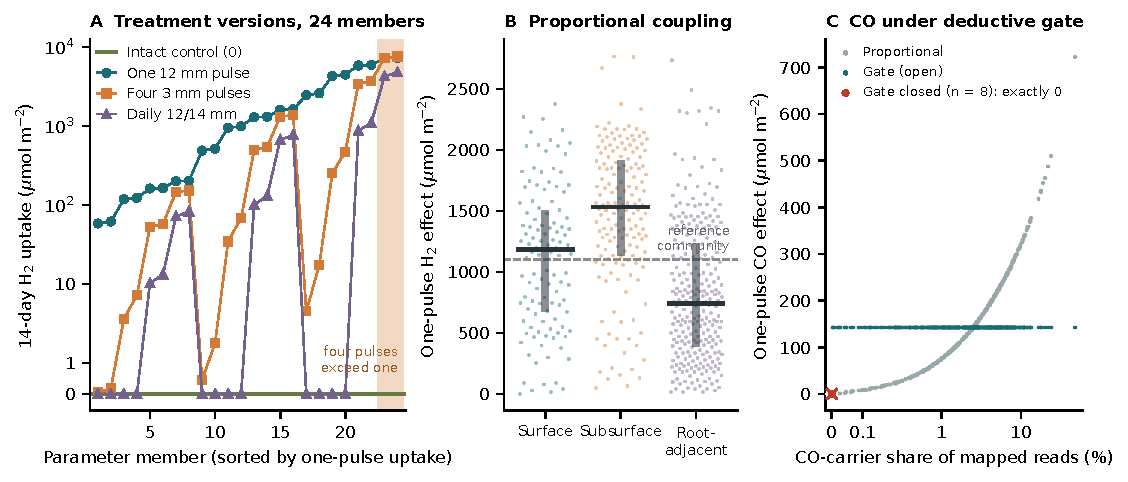
\includegraphics[width=\textwidth]{figures/v06_scenarios.pdf}
\caption{Causal scenarios under treatment versions and community coupling. (A) Fourteen-day hydrogen uptake for three schedules that each add 12~mm of water and for the untreated control, across \VersionMembers{} parameter members ordered by single-pulse uptake. (B) Single-pulse effect on hydrogen uptake for each sampled community when the rate coefficient is assumed proportional to hydrogenase-carrier share; bars show medians and interquartile ranges, and the dashed line the reference community. (C) Single-pulse effect on CO uptake against CO-carrier share. Under the deductive gate, communities without mapped CO carriers have zero effect in every regime.}
\label{fig:scenarios}
\end{figure}

\subsection{Identification with deductive closure}
The identification module unrolls the graph over time, computes the deductive value closure of an observed stratum, and evaluates the three rules of the $\mathrm{do}$-calculus on the mutilated graphs with the closure-augmented conditioning set. Only quantities that every admissible regime leaves unsevered can enter the closure, and a test confirms that no admissible target is ever closed. Table~\ref{tab:identification} lists the three derivations reported in the main text; each symbolic result is also checked numerically against the process model. In the same stratum of zero CO-carrier share, hydrogen uptake becomes independent of the CO pathway, whose oxygen demand otherwise couples the two gases.

{\small\setlength{\tabcolsep}{3pt}\begin{longtable}{@{}p{3.6cm}p{1.8cm}p{1.8cm}p{4.2cm}p{3.6cm}@{}}
\caption{Identification queries. Columns give the result of ordinary $d$-separation, the result with the closure-augmented conditioning set, the adjustment set and the verdict.}\label{tab:identification}\\\toprule
Query & Plain graph & With closure & Adjustment & Verdict\\\midrule\endfirsthead
\toprule Query & Plain graph & With closure & Adjustment & Verdict\\\midrule\endhead
\IdentificationRows
\bottomrule
\end{longtable}}

These are properties of the implementation under its equations. The identification of effects from data depends on the empirical adequacy of each mechanism, which the external tests evaluate. The Boolean natural-deduction results available for stratified causal--ontological theories motivate the design, and the continuous equations of the twin are checked by executable assertions and numerical tests. In the worked reaction-admission example, the controlled ablation changes the admitted network by supplying unsupported CO oxidation and illustrates the consequence of an additional biological assumption.

\subsection{Admissibility of every node}
Of the \GraphNodes{} represented quantities, \AdmissibleNodes{} are admissible intervention targets: \AdmissibleInputs{} exogenous inputs (water addition, salt in added water, evaporation demand, temperature, porosity, entry potential and retention exponent) and \AdmissibleStates{} states with a physical handle (the water and salt inventories). Table~\ref{tab:admissibility} lists the admissibility verdict for every node of the graph.

{\small\setlength{\tabcolsep}{3pt}\begin{longtable}{@{}lp{2.8cm}lp{1.3cm}p{6.2cm}@{}}
\caption{Admissibility of every node in the causal--ontological graph. Zones: ontological, evidence, deduced, exogenous (manipulable or fixed), constitutive and causal.}\label{tab:admissibility}\\\toprule
Node & Zone & Manipulable & Verdict & Reason\\\midrule\endfirsthead
\toprule Node & Zone & Manipulable & Verdict & Reason\\\midrule\endhead
\AdmissibilityRows
\bottomrule
\end{longtable}}

\section{Temporal prediction and external-transfer detail}\label{sec:transfer}
\subsection{Temporal prediction of molecular observations}
Repeated sampling supports prediction of subsequent molecular observations. Across \TestVisits{} future-campaign visits at 58 sites, geographic and seasonal ridge regression reduced RMSE relative to persistence by 0.055 on the $\log(1+\mathrm{GE})$ scale, with a site-bootstrap interval of 0.019--0.091. Its difference from a compartment mean was small and unresolved, and nominal 90\% residual intervals covered \ConformalCoverage{} of future observations. Compartment structure therefore explains much of the predictable variation in this observation layer, and predictions of physical flux require the separate evaluation of the process mechanisms reported in the main text. Forecasts and compartment contrasts are associational.

Biological replicates are averaged within site--compartment--campaign visits. Ridge regression with penalty 10 predicts $\log(1+\mathrm{GE})$ from training-standardized latitude and longitude, annual sine and cosine of collection day and one-hot compartment. Baselines are the global mean, the compartment mean and the latest site--compartment observation, with a compartment or global fallback at unseen locations. Each test campaign uses training observations collected before its first sample. The reference annotation catalogue is fixed retrospectively across all campaigns, and the forecast therefore holds out later campaigns of a fixed source catalogue. Table~\ref{tab:backtest} reports RMSE on $\log(1+\mathrm{GE})$, with nominal 90\% interval coverage for ridge regression.

Nominal 90\% intervals use absolute residuals from up to five site-held-out training folds, with empirical quantile level $\min\{1,\lceil(n+1)0.9\rceil/n\}$ for $n$ training visits. Fewer than two training sites cause an explicit error. These pooled cross-validation residuals centre intervals on a refit model, and dependence and temporal shift preclude a distribution-free coverage guarantee. Because held-out calibration sites have no persistence history, persistence uses its compartment or global fallback within these calibration folds. We report empirical coverage by campaign and compartment. Paired model-error comparisons (Table~\ref{tab:paired}) resample sites with all their visits, using 2,000 percentile-bootstrap draws and seed 42. Matched ecological contrasts use the same resampling unit after averaging replicates within site and campaign.
\begin{table}[ht]\centering\small
\caption{Future-campaign molecular prediction.}\label{tab:backtest}\begin{tabular}{rrrrrrr}\toprule
Campaign & Visits & Ridge & Persistence & Comp. mean & Global mean & Coverage\\\midrule
\BacktestRows
\bottomrule\end{tabular}\end{table}
\begin{table}[ht]\centering\small
\caption{Ridge-minus-baseline RMSE differences with site-bootstrap 95\% intervals.}\label{tab:paired}\begin{tabular}{lrr}\toprule
Baseline & Difference & Interval\\\midrule
\PairedRows
\bottomrule\end{tabular}\end{table}

\subsection{Namib hydration}
In Namib Desert microcosms, 400~$\mu$L of added water increased atmospheric hydrogen oxidation in the two fog-zone soils with quantified dry and wet rates. Mean wet-to-dry ratios were 41.3 (within-site bootstrap 95\% interval 31.1--56.0) at C14-2 and 19.4 (15.6--24.0) at C14-4. Hydrated microcosms from all ten sites reached sub-atmospheric hydrogen concentrations, while eight sites had no quantified dry atmospheric-rate endpoint within the reported observation period. The eight unquantified dry endpoints are retained in the site denominator but supply no numerical dry rate or fold change. In Namib, the dry and wet conditions use distinct subsamples. The publisher's rounded headspace gas amount reproduces the reported mass-normalized rates to within five parts per million. Historical field water potentials in this study describe a different temporal and experimental support from the incubation bottles, so the observations evaluate the combined retention--activation parameterization.

The predicted direction depends on the assumed bulk density. At 1.2 and 1.5~g~cm$^{-3}$ the reference model predicts higher hydrated than dry uptake at all ten sites. At 1.8~g~cm$^{-3}$, the hydrated C14-2 soil (gravimetric water content 0.218~g~g$^{-1}$) reaches a volumetric water content of 0.39 against porosity 0.40; the predicted dry flux (0.277) then exceeds the hydrated flux (0.0046, both in the model's areal units), whereas the other nine sites retain the positive direction. The direction itself therefore depends on an unmeasured soil property. The reference model also predicts zero dry uptake at the two active fog sites, which exposes a failure of those assumptions.

\subsection{Sonoran incubations and field measurements}
Across four soil-source plots at one residence, increasing gravimetric water content from 0.02 to 0.20~g~g$^{-1}$ increased mean hydrogen uptake by 0.37--0.55~nmol~m$^{-2}$~s$^{-1}$. Uptake also increased from 0.10 to 0.20~g~g$^{-1}$ in every plot, by 0.32--0.51~nmol~m$^{-2}$~s$^{-1}$. With the reference retention relation and an assumed bulk density of 1.5~g~cm$^{-3}$, the twin instead predicts a decline over this upper interval. The sign of the wetting response therefore leaves the transferable parameter values untested. The source data include small net emissions at dry or intermediate moisture, and these observations retain their sign. Source-batch bootstrap intervals characterize the sampled plots, and the four plots belong to one residence.

In the field comparison, the calibrated model improved on the training mean in three of four held campaigns, with a larger error in August. Every training split selected the no-temperature-amplification member, $Q_{10}=1$, and the largest tested porosity and retention exponent. The Sonoran field grid contains 54 combinations of porosity, retention exponent, entry potential and temperature response. A kinetic coefficient is fitted separately within each combination and training fold, and training selects the best member before applying it to the held campaign. All four selected members have porosity 0.5, retention exponent 6 and $Q_{10}=1$; entry potential is $-0.001$~MPa when June is held out and $-0.01$~MPa in the other folds. These grid boundaries mark an unresolved sensitivity of the calibration, and the grid supplies point selections without uncertainty intervals on measured soil properties. Both the fixed and calibrated models assume that the reported sensor measurements represent a homogeneous active soil layer. These results identify environmental parameterization as a prerequisite for useful transfer in this one-site seasonal comparison. An independent implementation of the diffusion--reaction equation recomputes all 96 Sonoran field predictions and checks the source aggregation, corrected flux column, fold boundaries and error metrics. The source hashes and generated table hashes are recorded in the reproduction manifest.

\subsection{Transfer among temperate soils}
Transfer among contrasting temperate environments was uneven. We fitted a common response amplitude on two of the forest, meadow and sand soils of the temperate study and predicted the third. The activation--diffusion envelope improved held-soil bottle-rate RMSE over both diffusion-only and training-mean alternatives for forest and sand, and gave a larger error for meadow. This test extends the within-soil, held-replicate comparison, which is retained as a development comparison, to an environmental shift, while the study still informs the activation threshold. Together, the external results support water-dependent activation as a useful mechanism whose quantitative expression depends on soil and measurement context. The evaluation is retrospective, because the published conclusions were known when the analysis protocol was fixed.

\section{Composition with external models}\label{sec:composition}
The composition runner evaluates 12 management what-if chains against the 14-day single-pulse rain baseline (12~mm rain on day 0, initial water storage 1.8~mm, soil temperature $25~^\circ$C, potential evaporation 1~mm~day$^{-1}$; reference uptake 1,102.3~$\mu$mol~H$_2$~m$^{-2}$ and 144.4~$\mu$mol~CO~m$^{-2}$). Every uncertainty envelope in this section is the one-at-a-time constant envelope at the reference twin parameters: each external constant takes its low and high value in turn, and the twin process parameters stay at their reference values. The joint uncertainty analysis of Section~\ref{sec:uq} varies all constants and twin parameters together. Table~\ref{tab:constants} lists the constants, Table~\ref{tab:envelopes} and Fig.~\ref{fig:v07_composition} summarize all 12 experiments with their one-at-a-time envelopes and endpoint provenance labels, and the subsections that follow give the chain specifications, the one-at-a-time results and the field-trial comparison.

\subsection{External constants registry and verification audit}
All 42 external constants used in the composition layer are recorded in a registry, and its digest is stored with every output. Each entry records a central value, low and high bounds, unit, source citation and a verification status from a manual audit against the cited sources. Table~\ref{tab:constants} lists them with their statuses: 23 constants are verified in source, 10 are modeller assumptions and 9 have a source that was not checked. The verified constants are the two leaching and conductivity conversion factors, the eight Maas--Hoffman crop thresholds and slopes, the Julian year length, the tropospheric hydrogen background, the potential-evaporation warming scaling, and the ten Hada Al-Sham field-trial constants and digitised ratios. The modeller assumptions are the two crop water demands, the full-cover organic-mulch evaporation reduction, the biocrust carbon-fixation context value, the solar-panel soil cooling, evaporation reduction and washing interval, the cloud-seeding rainfall enhancement, the off-road compaction $e$-folding pass scale, and the soil-to-air warming pass-through. The constants whose source was not checked are the NaCl molarity per unit conductivity, the shade-net soil cooling, the biochar porosity slope, the knallgas CBB stoichiometry, the carbon molar mass, the hydrogen-economy global hydrogen mixing ratio, the panel-washing water volume, the quartz particle density and the asymptotic off-road bulk-density increase.

{\footnotesize\setlength{\tabcolsep}{3pt}\begin{longtable}{@{}rp{3.9cm}p{3.1cm}p{2.5cm}p{3.1cm}p{2.1cm}@{}}
\caption{External constants of the composition layer. Columns give the readable name, the central value with its low and high bounds, the unit, the source and the verification status from the audit against the cited source.}\label{tab:constants}\\\toprule
\# & Constant & Value [low, high] & Unit & Source & Status\\\midrule\endfirsthead
\toprule \# & Constant & Value [low, high] & Unit & Source & Status\\\midrule\endhead
\ConstantRows
\bottomrule
\end{longtable}}

Six corrections were applied to the registry during source verification before the final experiments. The DOI of Novelli et al. (1999) for the background hydrogen mixing ratio (0.53~ppm) was corrected to doi:10.1029/1999JD900788. The tomato salinity slope was re-centred to 9.5\%~dS$^{-1}$~m with bounds 9.0 to 9.9\%~dS$^{-1}$~m; the lower bound comes from the FAO evapotranspiration paper, and the upper bound is the value usually attributed to Maas and Hoffman, which remains unchecked. The source citations for the Maas--Hoffman slopes of alfalfa (7.3\%~dS$^{-1}$~m), date palm (3.6\%~dS$^{-1}$~m) and barley (5.0\%~dS$^{-1}$~m) were updated to the FAO evapotranspiration paper (Table~23). The low and high bounds of the leaching concentration factor (central 1.5) were set to 1.0 and 2.1 from the concentration factors for 30\% and 10\% leaching fractions. The upper bound of the evaporation scaling per degree (central 0.04~$^\circ$C$^{-1}$) was adjusted to 0.06~$^\circ$C$^{-1}$ to match the Clausius--Clapeyron ceiling in Scheff and Frierson (2014). The citation for the mulch evaporation reduction (0.5) was corrected to Chapter~9 of the FAO evapotranspiration paper, and its status was set to modeller assumption as a linear extrapolation of the 5\% evaporation reduction per 10\% organic-mulch cover rule.

\subsection{Chain specifications and one-at-a-time envelopes}
Each experiment in Table~\ref{tab:envelopes} wires upstream management translations, the twin intervention runner and downstream response models through typed ports.

\begin{table}[ht]\centering\small\setlength{\tabcolsep}{3pt}
\caption{Summary of the 12 management what-if compositions on the 14-day single-pulse reference baseline, with one-at-a-time uncertainty envelopes across referenced external constants at reference twin parameters, and endpoint provenance labels.}\label{tab:envelopes}
\begin{tabular}{@{}rp{2.3cm}p{5.0cm}p{3.1cm}p{2.1cm}p{1.8cm}@{}}
\toprule
\# & Experiment & Headline & Central [low, high] & Unit & Provenance \\
\midrule
1 & Brackish irrigation & Alfalfa relative yield at 8 dS m$^{-1}$, daily irrigation & 0.887 [0.8, 0.938] & fraction & external model \\
2 & Drip or flood & H$_2$ uptake change, irrigation every 10 days & $-$5.55 [$-$5.55, $-$5.55] & \% of baseline & twin \\
3 & Mulch and shade & H$_2$ uptake change, full mulch cover & 50.1 [36.3, 53.9] & \% of baseline & twin \\
4 & Biochar & H$_2$ uptake change, 5\% w/w biochar & $-$2.26 [$-$4.24, $-$0.641] & \% of baseline & twin \\
5 & Inoculation & CO uptake after 1\% CO-carrier inoculation of a closed-gate sample & 144 [144, 144] & $\mu$mol m$^{-2}$ & twin \\
6 & Carbon fixation bound & Upper bound of carbon fixed by hydrogen oxidizers, sample with the highest autotroph share & 0.0576 [0.0345, 0.0864] & g C m$^{-2}$ yr$^{-1}$ & external model \\
7 & Hydrogen leakage & H$_2$ uptake change at twice the background mixing ratio & 100 [100, 100] & \% of baseline & twin \\
8 & Solar park & H$_2$ uptake change, full panel cover & 16.6 [$-$1.9, 30.5] & \% of baseline & twin \\
9 & Cloud seeding & H$_2$ uptake change, full-intensity seeding (+10\% rain on rain days) & 12.7 [0, 24.7] & \% of baseline & twin \\
10 & Vehicle compaction & H$_2$ uptake change, 50 passes & $-$1.49 [$-$7.58, 1] & \% of baseline & twin \\
11 & Climate warming & H$_2$ uptake change, +4 $^\circ$C with unchanged rainfall & 7.16 [0.245, 15.1] & \% of baseline & twin \\
12 & Inoculated alfalfa & Inoculated alfalfa relative yield at 7.81 dS m$^{-1}$, salinity fitted to the field trial (fresh weight) & 0.915 [0.891, 0.936] & fraction & external model \\
\bottomrule
\end{tabular}

\end{table}

\begin{figure}[!htbp]
\centering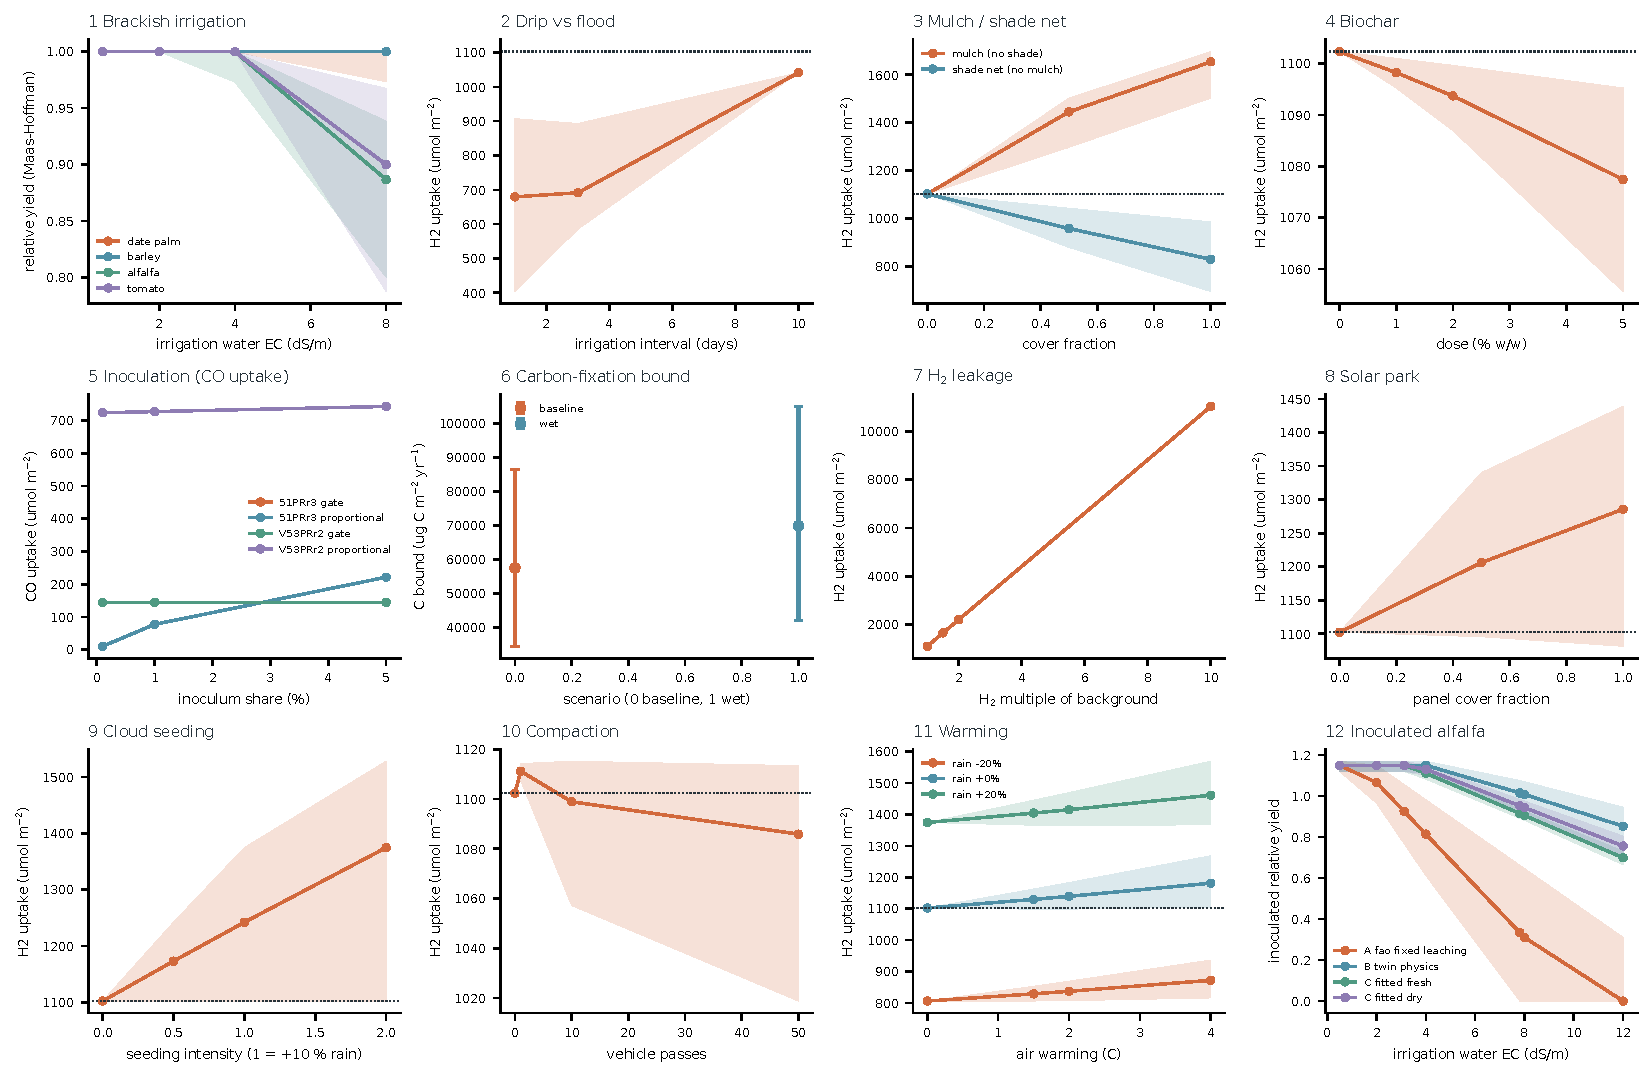
\includegraphics[width=\textwidth]{figures/v07_composition.pdf}
\caption{Small-multiples summary of the 12 management what-if compositions on the 14-day single-pulse reference baseline. Panels display central predictions (lines and points), one-at-a-time uncertainty envelopes across referenced external constants at reference twin parameters (shaded bands and error bars) and the rain-only baseline (dotted horizontal line where applicable).}\label{fig:v07_composition}
\end{figure}

In the brackish irrigation experiment, upstream models convert irrigation water conductivity to NaCl concentration, set the irrigation schedule and add a generic crop water demand (6~mm~day$^{-1}$). They deliver daily water and NaCl to the twin across irrigation conductivities of 0.5, 2, 4 and 8~dS~m$^{-1}$. Downstream models convert the twin's soil-solution salinity to root-zone conductivity and compute relative yield for date palm, barley, alfalfa and tomato with the Maas--Hoffman response. The high-salinity constant-envelope runs at 8~dS~m$^{-1}$ exceed the 0.1~mol~L$^{-1}$ dilute osmotic domain.

In the drip or flood experiment, a generic crop water demand (6~mm~day$^{-1}$) and an irrigation schedule deliver equal seasonal water demand on 1-, 3- or 10-day intervals on top of the 12~mm rain pulse, and the twin integrates 14-day hydrogen and CO uptake. In the mulch and shade experiment, upstream models scale daily evaporation demand and offset soil temperature across mulch fractions of 0, 0.5 and 1 and shade levels of 0, 0.5 and 1; full mulch with shade increases 14-day hydrogen uptake by 14.1\% ($-3.94$ to 34.8\%). In the biochar experiment, an upstream model adds 0.006 to soil porosity per percentage point w/w across 0, 1, 2 and 5\% biochar, which raises $\phi$ from 0.40 to 0.43 at 5\% w/w, and the twin evaluates the resulting change in matric potential, diffusivity and hydrogen uptake.

In the inoculation experiment, an upstream model mixes a CO-carrier MAG or a non-carrier MAG at shares of 0.1\%, 1\% and 5\% into a sample with a closed CO gate or a sample with an open CO gate, recomputes the CO community factor under the gate and proportional couplings and runs the twin. In the carbon fixation experiment, twin 14-day hydrogen and CO uptake feed a downstream knallgas model, which is gated by the hydrogen-autotroph candidate class and uses the stoichiometry of 1/6~mol~CO$_2$ per mol~H$_2$ of Bongers (1970), and a CO-oxidation carbon balance, which is fed by twin CO uptake gated by the CO-oxidizer class. The experiment covers the sample with the highest autotroph share and a sample without entailed autotrophic candidates. In the hydrogen leakage experiment, an upstream model scales the twin's exogenous atmospheric hydrogen forcing across 1, 1.5, 2 and 10 times the 0.53~ppm background (Novelli et al. (1999)) and records hydrogen uptake, CO uptake and the peak ratio of oxygen demand to supply.

In the solar park experiment, upstream models apply under-panel cooling, evaporation reduction and 14-day wash pulses across panel cover fractions of 0, 0.5 and 1 before the twin runs. In the cloud seeding experiment, an upstream model multiplies existing rain pulses by $1+0.10\,s$ across seeding intensities $s\in\{0,0.5,1,2\}$. In the compaction experiment, an upstream model increases bulk density from 1.59~g~cm$^{-3}$ toward an asymptotic increment of 0.25~g~cm$^{-3}$ across 0, 1, 10 and 50 vehicle passes (Webb (1983)), converts bulk density to porosity at a quartz particle density of 2.65~g~cm$^{-3}$ and runs the twin. In the warming experiment, an upstream model crosses air warming offsets of 0, 1.5, 2 and 4~$^\circ$C with rainfall scaling of $-20\%$, 0\% and $+20\%$, and scales potential evaporation by 4\%~$^\circ$C$^{-1}$ (Scheff and Frierson (2014)) before the twin runs. In the inoculated alfalfa experiment, three alternative root-zone salinity models (Models A, B and C of Section~\ref{sec:hada}) feed the Maas--Hoffman alfalfa response and the SA187 yield benefit across irrigation conductivities of 0.5, 2, 3.12, 4, 7.81, 8 and 12~dS~m$^{-1}$.

\subsection{One-at-a-time results}
Adding irrigation water (6~mm~day$^{-1}$ seasonal demand) on top of the rain pulse reduces soil hydrogen uptake because sustained pore moisture restricts Millington--Quirk gas diffusion once water potential exceeds the activation threshold. At reference twin parameters, daily drip irrigation changes 14-day hydrogen uptake by $-38\%$ (one-at-a-time constant envelope $-63.4$ to $-17.7\%$), compared with $-37.3\%$ for 3-day pulses and $-5.55\%$ for 10-day flood pulses. Under daily brackish irrigation from 0.5 to 8~dS~m$^{-1}$, twin hydrogen uptake declines by 38.4\% to 43.9\% as accumulated salt lowers osmotic potential, and the high-salinity envelope runs at 8~dS~m$^{-1}$ exceed the 0.1~mol~L$^{-1}$ dilute domain. Downstream Maas--Hoffman relative yield at 8~dS~m$^{-1}$ is 0.887 (0.800 to 0.938) for alfalfa, 1.00 for barley, 1.00 (0.973 to 1.00) for date palm and 0.900 (0.787 to 0.967) for tomato. Across the remaining physical chains, full organic mulch changes 14-day hydrogen uptake by 50.1\%, solar-panel cover with 14-day washing by 16.6\%, cloud seeding (+10\% rain on rain days) by 12.7\%, +4~$^\circ$C warming at unchanged rainfall by 7.16\%, shade-net cooling ($-5~^\circ$C) by $-24.8\%$, 5\% w/w biochar by $-2.26\%$ and 50 off-road vehicle passes by $-1.49\%$ (envelopes in Table~\ref{tab:envelopes} and Fig.~\ref{fig:v07_composition}).

Perturbing atmospheric hydrogen above the 0.53~ppm background scales the 14-day soil hydrogen sink linearly across 1.5, 2 and 10 times background (+50\%, +100\% and +900\% uptake, reaching 11,023~$\mu$mol~m$^{-2}$ at 5.3~ppm), because first-order reaction--diffusion is proportional to surface concentration. Peak oxygen demand reaches only 0.00073\% of diffusive oxygen supply, which leaves oxygen unlimiting and CO uptake unchanged at 144.4~$\mu$mol~m$^{-2}$. Chaining twin hydrogen uptake to the knallgas CBB stoichiometry (1/6~mol~CO$_2$ per mol~H$_2$) under the deductive gate gives an annualised carbon-fixation upper bound in the sample with the highest autotroph share (2.64\% autotroph share) of 0.058~g~C~m$^{-2}$~yr$^{-1}$ (envelope 0.035 to 0.086~g~C~m$^{-2}$~yr$^{-1}$; 183.7~$\mu$mol~CO$_2$~m$^{-2}$ over 14 days), equivalent to 0.58\% of a 10~g~C~m$^{-2}$~yr$^{-1}$ dryland biocrust reference flux. In a sample where the entailed hydrogen-autotroph share is 0\%, the downstream deductive gate returns 0 fixed carbon with deduced provenance while twin hydrogen oxidation continues (1,102.3~$\mu$mol~m$^{-2}$ under the gate). Coupled CO oxidation converts CO to CO$_2$ in equimolar stoichiometry with 0 net change in atmospheric carbon atoms.

Inoculation acts as a constitutive intervention that recomputes deduced community shares at fixed ontology and genome annotations before the causal mechanisms run. In a sample with 0\% mapped CO-carrier share and a closed CO gate (0~$\mu$mol~m$^{-2}$ uptake), introducing a CO-carrier MAG at 0.1\%, 1\% or 5\% share opens the gate and increases 14-day CO uptake to 144.4~$\mu$mol~m$^{-2}$ under gate coupling, or to 10.4, 77.4 and 221.4~$\mu$mol~m$^{-2}$ under proportional coupling. Introducing a non-carrier MAG into this sample keeps CO uptake at 0~$\mu$mol~m$^{-2}$. Introducing the CO carrier into a sample whose gate is already open (47.8\% initial share) gives 0 change under gate coupling and raises proportional CO uptake from 723.3 to 723.7, 727.2 and 742.9~$\mu$mol~m$^{-2}$ across the same shares.

\subsection{Hada Al-Sham field-trial digitisation and root-zone salinity models}\label{sec:hada}
To compare the composed salinity chains against the Hada Al-Sham alfalfa field trial irrigated at 3.12 and 7.81~dS~m$^{-1}$ with and without \textit{Enterobacter} sp. SA187 (de Z{\'e}licourt et al. (2018), doi:10.1371/journal.pgen.1007273), we digitised Fig.~1 of the published article. In each panel, the digitiser detects the horizontal y-axis tick marks from 0 to 14~t~ha$^{-1}$ (step 2~t~ha$^{-1}$) at pixel column $x=156$ and fits a linear pixel-to-yield calibration by ordinary least squares, with a maximum calibration residual of 0.0148~t~ha$^{-1}$ in the low-salinity panel and 0.0131~t~ha$^{-1}$ in the high-salinity panel. Bar-top pixel rows are converted to t~ha$^{-1}$ for mock and SA187-inoculated bars across both traits (fresh weight and dry biomass) and both growing seasons. Cross-checking the digitised bar heights against all 8 SA187 percentage increases printed on the figure (+16\% and +12\% fresh and +14\% and +17\% dry at 3.12~dS~m$^{-1}$; +15\% and +12\% fresh and +13\% and +17\% dry at 7.81~dS~m$^{-1}$) reproduces all 8 printed percentages within 0.83 percentage points (maximum relative difference 0.0083). Digitised season-1 mock yields at 3.12 and 7.81~dS~m$^{-1}$ are 5.411 and 4.306~t~ha$^{-1}$ for fresh weight (high-to-low ratio 0.7958, digitisation envelope 0.7779 to 0.8141) and 2.072 and 1.716~t~ha$^{-1}$ for dry biomass (ratio 0.8282, 0.8018 to 0.8554). Subsequent-season yields are recorded in the digitised archive and excluded from salinity-ratio fitting because exceptional rainfall confounded the high-salinity treatment in the second season.

Three root-zone salinity formulations were chained to the Maas--Hoffman alfalfa response (threshold 2.0~dS~m$^{-1}$, slope 7.3\%~dS$^{-1}$~m) and the SA187 yield multiplier ($b=0.15$, range 0.12 to 0.17).

Model~A uses the standard fixed leaching factor $\mathrm{EC_e}=1.5\,\mathrm{EC_w}$ (range 1.0 to 2.1 across 30\% to 10\% leaching fractions). At 3.12 and 7.81~dS~m$^{-1}$, implied $\mathrm{EC_e}$ is 4.68 and 11.72~dS~m$^{-1}$, predicting a mock high-to-low yield ratio of 0.362 (0.00 to 0.627; gap $-0.434$ fresh and $-0.467$ dry) and an inoculated relative yield at 7.81~dS~m$^{-1}$ of 0.334 (0.00 to 0.662).

Model~B runs the twin's bare-sand water and salt balance under daily irrigation at 8~mm~day$^{-1}$ and converts mean soil-water conductivity via $\mathrm{EC_e}=\mathrm{EC_{sw}}/2$. With 1~mm~day$^{-1}$ bare-soil evaporation and no crop transpiration, drainage keeps implied $\mathrm{EC_e}$ at 1.44~dS~m$^{-1}$ for $\mathrm{EC_w}=3.12$~dS~m$^{-1}$, predicting a mock yield ratio of 0.883 (0.795 to 0.935; gap +0.087 fresh and +0.055 dry) and an inoculated relative yield at 7.81~dS~m$^{-1}$ of 1.015 (0.914 to 1.076), while twin gas uptake abstains at $\mathrm{EC_w}=12$~dS~m$^{-1}$ outside the 0.1~mol~L$^{-1}$ dilute NaCl domain.

Model~C fits $f$ in $\mathrm{EC_e}=f\,\mathrm{EC_w}$ so that the Maas--Hoffman mock yield ratio between 7.81 and 3.12~dS~m$^{-1}$ matches the digitised first-season mock ratio, yielding $f=0.614$ (0.582 to 0.648) for fresh weight and $f=0.557$ (0.510 to 0.604) for dry biomass. At $\mathrm{EC_w}=3.12$~dS~m$^{-1}$, these fitted factors imply root-zone $\mathrm{EC_e}=1.92$~dS~m$^{-1}$ (1.82 to 2.02~dS~m$^{-1}$, fresh) and $1.74$~dS~m$^{-1}$ (1.59 to 1.88~dS~m$^{-1}$, dry), which matches the measured site soil conductivity of 1.95~dS~m$^{-1}$, and predict inoculated relative yields at 7.81~dS~m$^{-1}$ of 0.915 (0.891 to 0.936) for fresh weight and 0.952 (0.922 to 0.984) for dry biomass. With the fitted fresh-weight leaching factor and the 15\% (12 to 17\%) SA187 yield multiplier, the predicted inoculated relative yield at 7.81~dS~m$^{-1}$ is 0.915 (one-at-a-time envelope 0.891 to 0.936). A single trial at two salinities identifies the SA187 benefit only as a constant multiplier across the tested 3.12 to 7.81~dS~m$^{-1}$ range.

\section{Uncertainty quantification}\label{sec:uq}
Joint parameter-uncertainty propagation and global sensitivity analysis evaluate 14 management and community questions across 111 scenario levels and 1,383 output series. Table~\ref{tab:v08_parameters} lists all 13 uncertain twin process parameters, each carrying the verification status modeller assumption. For each scenario level, the active input vector combines these twin parameters (excluding $\phi$ when porosity is directly set by the biochar or compaction upstream model) with the constants referenced by the level's upstream and downstream models from the registry of Section~\ref{sec:composition} (42 constants in total, each assigned a triangular distribution over its low, central and high values).

\begin{table}[!htbp]\centering\small\setlength{\tabcolsep}{3pt}
\caption{Twin process-parameter uncertainty registry. All 13 parameters carry the verification status modeller assumption; porosity is excluded from sampling in levels where the intervention directly clamps soil porosity.}\label{tab:v08_parameters}
\begin{tabular}{@{}rlp{1.9cm}p{4.1cm}p{1.4cm}p{3.1cm}@{}}
\toprule
\# & Parameter & Distribution & Reference [low, high] & Unit & Status \\
\midrule
1 & H$_2$ rate constant $k_{\mathrm{H_2}}$ & loguniform & 0.001 [0.0001, 0.01] & s$^{-1}$ & modeller assumption \\
2 & CO rate constant $k_{\mathrm{CO}}$ & loguniform & 0.001 [0.0001, 0.01] & s$^{-1}$ & modeller assumption \\
3 & air-entry potential $\psi_e$ & loguniform & $-$0.001 [$-$0.01, $-$0.0001] & MPa & modeller assumption \\
4 & retention exponent $b$ & triangular & 4 [2, 6] & -- & modeller assumption \\
5 & full-activation potential $\psi_w$ & loguniform & $-$0.1 [$-$0.3, $-$0.03] & MPa & modeller assumption \\
6 & activation threshold $\psi_d$ & triangular & $-$85 [$-$100, $-$70] & MPa & modeller assumption \\
7 & activation shape $a$ & triangular & 1 [0.5, 2] & -- & modeller assumption \\
8 & temperature coefficient $Q_{10}$ & uniform & 2 [1, 2] & -- & modeller assumption \\
9 & free-air diffusivity (H$_2$) & triangular & $7.7\times10^{-5}$ [$6.16\times10^{-5}$, $9.24\times10^{-5}$] & m$^2$ s$^{-1}$ & modeller assumption \\
10 & free-air diffusivity (CO) & triangular & $2.1\times10^{-5}$ [$1.68\times10^{-5}$, $2.52\times10^{-5}$] & m$^2$ s$^{-1}$ & modeller assumption \\
11 & drainage fraction & triangular & 0.5 [0.3, 0.7] & day$^{-1}$ & modeller assumption \\
12 & field-capacity fraction & triangular & 0.5 [0.4, 0.6] & -- & modeller assumption \\
13 & porosity $\phi$ & triangular & 0.4 [0.35, 0.5] & -- & modeller assumption \\
\bottomrule
\end{tabular}

\end{table}

Table~\ref{tab:v08_uq} and Fig.~\ref{fig:v08_sensitivity} report the central prediction, median, joint 5--95\% parameter-uncertainty interval, top two individual total-order Sobol' contributors ($S_T$) and modeller-assumption group total-order index ($S_T^{\mathrm{assum}}$) for the headline level and output of each of the 14 questions. For the doubling of atmospheric hydrogen ($2\times$ background H$_2$), the relative H$_2$ uptake change is $+100\%$ across every parameter draw (5--95\% interval $100\%$ to $100\%$) because the first-order reaction--diffusion equation is linear in surface concentration. The Sobol' indices in Table~\ref{tab:v08_uq} and Fig.~\ref{fig:v08_sensitivity} for this question are therefore reported on the paired 14-day H$_2$ uptake contrast (central $1,102.3~\mu$mol~m$^{-2}$, median $937.7$, 5--95\% interval $122.6$ to $4,768.4~\mu$mol~m$^{-2}$, where the H$_2$ rate constant has $S_T=0.882$ and the retention exponent has $S_T=0.130$). In the questions on missing CO genes and carbon fixation, samples with a closed deductive gate return exact 0 with interval $[0,0]$ and deduced provenance.

\begin{table}[!htbp]\centering\scriptsize\setlength{\tabcolsep}{3pt}
\caption{Headline joint parameter-uncertainty summary across the 14 questions. Columns give the central prediction at reference parameters, the Monte Carlo median and 5--95\% interval, the top two individual total-order Sobol' contributors ($S_T$) and the total-order group index of modeller-assumption inputs ($S_T^{\mathrm{assum}}$).}\label{tab:v08_uq}
\begin{tabular}{@{}rp{2.0cm}p{3.2cm}rp{2.6cm}p{4.3cm}r@{}}
\toprule
\# & Question & Headline level (unit) & Central & Median [5\%, 95\%] & Top two $S_T$ contributors & $S_T^{\mathrm{assum}}$ \\
\midrule
1 & rain-pattern & Four 3 mm showers (\%) & $-$63.2 & $-$68.7 [$-$100, $-$2.77] & \texttt{retention\_\allowbreak{}b} (0.687), \texttt{psi\_\allowbreak{}entry\_\allowbreak{}mpa} (0.258) & 0.995 \\
2 & drip-or-flood & every 10 d (\%) & $-$5.55 & 2.48 [$-$47.9, 175] & \texttt{psi\_\allowbreak{}entry\_\allowbreak{}mpa} (0.611), \texttt{retention\_\allowbreak{}b} (0.396) & 0.975 \\
3 & cloud-seeding & intensity 1 (\%) & 12.7 & 12.8 [3.6, 31.2] & \texttt{cloud\_\allowbreak{}seeding\_\allowbreak{}rain\_\allowbreak{}increase\_\allowbreak{}frac} (0.426), \texttt{retention\_\allowbreak{}b} (0.288) & 0.981 \\
4 & salty-water & EC\_w=8 dS/m (\%) & $-$43.9 & $-$37.1 [$-$74.9, 95.3] & \texttt{retention\_\allowbreak{}b} (0.517), \texttt{psi\_\allowbreak{}entry\_\allowbreak{}mpa} (0.412) & 0.983 \\
5 & alfalfa-bacterium & C\_fitted\_fresh; EC\_w=7.81 (fraction) & 0.915 & 0.911 [0.887, 0.931] & \texttt{sa187\_\allowbreak{}mock\_\allowbreak{}ratio\_\allowbreak{}fresh} (0.515), \texttt{sa187\_\allowbreak{}benefit\_\allowbreak{}b} (0.364) & 0 \\
6 & hotter & +4 C, rain +0\% (\%) & 7.16 & $-$2.64 [$-$13.2, 9.97] & \texttt{q10} (0.752), \texttt{evap\_\allowbreak{}scaling\_\allowbreak{}per\_\allowbreak{}c} (0.148) & 0.854 \\
7 & mulch-shade & mulch 1, shade 0 (\%) & 50.1 & 50.1 [11.2, 91.8] & \texttt{retention\_\allowbreak{}b} (0.594), \texttt{psi\_\allowbreak{}entry\_\allowbreak{}mpa} (0.247) & 0.984 \\
8 & solar-park & panel cover 1 (\%) & 16.6 & 23.4 [0.352, 51.8] & \texttt{retention\_\allowbreak{}b} (0.407), \texttt{solar\_\allowbreak{}panel\_\allowbreak{}evap\_\allowbreak{}reduction\_\allowbreak{}frac} (0.289) & 1.05 \\
9 & compaction & 50 passes (\%) & $-$1.49 & 0.205 [$-$19, 40.3] & \texttt{k\_\allowbreak{}h2\_\allowbreak{}s} (0.359), \texttt{retention\_\allowbreak{}b} (0.341) & 0.988 \\
10 & biochar & 5 \% w/w (\%) & $-$2.26 & $-$2.03 [$-$12.8, 4.12] & \texttt{retention\_\allowbreak{}b} (0.423), \texttt{psi\_\allowbreak{}entry\_\allowbreak{}mpa} (0.272) & 0.955 \\
11 & missing-co-genes & V53PRr2 (CO gate open) ($\mu$mol m$^{-2}$) & 144 & 126 [21.1, 501] & \texttt{k\_\allowbreak{}co\_\allowbreak{}s} (0.839), \texttt{retention\_\allowbreak{}b} (0.14) & 1 \\
12 & adding-microbes & V53PRr2 (CO gate already open) + CO carrier; proportional; share 0.01 (\%) & 0.549 & 0.55 [0.545, 0.628] & \texttt{k\_\allowbreak{}co\_\allowbreak{}s} (0.912), \texttt{psi\_\allowbreak{}entry\_\allowbreak{}mpa} (0.083) & 1 \\
13 & air-hydrogen & 2x background (\%) & 100 & 100 [100, 100] & \texttt{k\_\allowbreak{}h2\_\allowbreak{}s} (0.882), \texttt{retention\_\allowbreak{}b} (0.13) & 1.01 \\
14 & carbon-fixation & baseline (12 mm pulse); F14Dr1 (g C m$^{-2}$ yr$^{-1}$) & 0.0576 & 0.0499 [0.00622, 0.269] & \texttt{k\_\allowbreak{}h2\_\allowbreak{}s} (0.829), \texttt{retention\_\allowbreak{}b} (0.125) & 0.964 \\
\bottomrule
\end{tabular}

\end{table}

The full Saltelli design ($N=1,024$ base samples, 500 bootstrap draws for 95\% Sobol' confidence intervals, 1,219 Slurm array tasks and 2,285,568 model evaluations) was checked for sample-size convergence by comparing the 5--95\% interval endpoints between the first $N/2=512$ base samples and all $N=1,024$ base samples. Seven non-discrete levels exceeded the 5\% interval-width shift threshold and were rerun at $N=2,048$ (171 array tasks). After the $N=2,048$ rerun, 7 of the 1,383 evaluated outputs remain flagged with half-$N$ endpoint shifts of 5.5\% to 10.3\% of the interval width, reflecting the heavy upper tail of the log-uniform reaction-rate constants. In a 25-task cross-machine verification check (20,011 scalar outputs), 315 raw floating-point values differed between workstations at a maximum relative difference of $2.0\times 10^{-11}$, and all published summaries are rounded to 6 significant digits.

\begin{figure}[!htbp]
\centering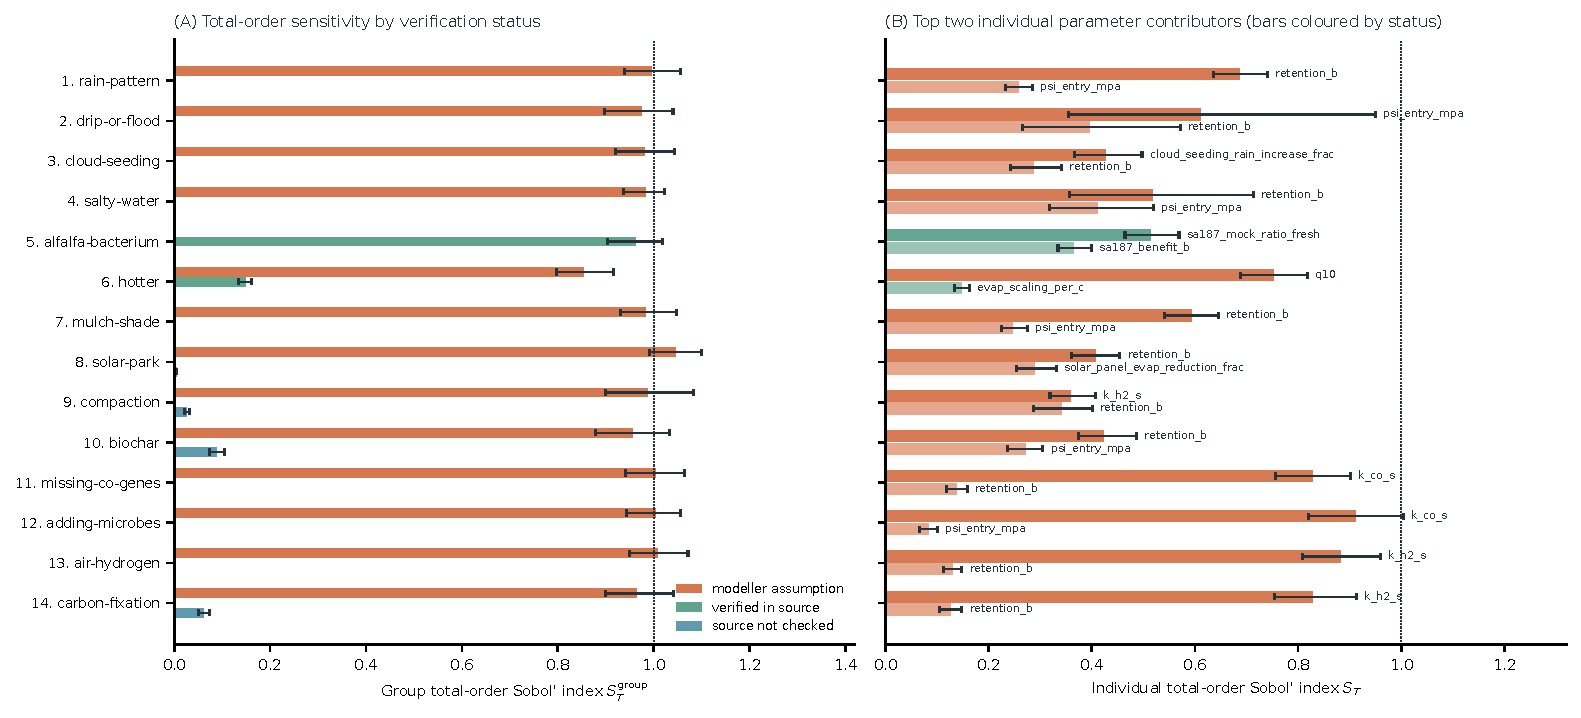
\includegraphics[width=\textwidth]{figures/v08_sensitivity.pdf}
\caption{Global sensitivity of the 14 headline question outputs under joint parameter uncertainty. (A) Group total-order Sobol' indices ($S_T^{\mathrm{group}}$ with 95\% bootstrap intervals) partitioned by input verification status (modeller assumption, verified in source and source not checked). (B) Top two individual parameter contributors ($S_T$ with 95\% bootstrap intervals) for each question, coloured by verification status.}\label{fig:v08_sensitivity}
\end{figure}

\subsection{Joint uncertainty of every intervention}
Propagating joint parameter uncertainty across all 14 management and community questions (\UQLevels{} scenario levels, \UQOutputs{} evaluated outputs and \UQEvaluations{} model evaluations at base sample size $N=1,024$) shows that absolute 14-day hydrogen uptake on the single-pulse baseline spans an order of magnitude (central \QBaseHtwoRef{}~$\mu$mol~m$^{-2}$, median \QBaseHtwoMedian{}, joint 5--95\% interval \QBaseHtwoLow{} to \QBaseHtwoHigh{}~$\mu$mol~m$^{-2}$), with variance dominated by the assumed reaction-rate constant $k_{\mathrm{H_2}}$ (total-order Sobol' index $S_T=\QBaseHtwoSTkHtwo$) and the Campbell retention exponent $b$ ($S_T=\QBaseHtwoSTb$). Paired percentage changes between intervened and baseline trajectories cancel the first-order rate scale and separate interventions with a consistent sign across at least 95\% of draws from those whose direction depends on the parameters.

Four 3~mm showers (\QRainFourRef\% central, median \QRainFourMedian\%, joint 5--95\% interval \QRainFourLow\% to \QRainFourHigh\%), daily 0.86~mm drizzle (\QRainDrizzleRef\% central, median \QRainDrizzleMedian\%, \QRainDrizzleLow\% to \QRainDrizzleHigh\%) and shade-net cooling (\QShadeFullRef\% central, median \QShadeFullMedian\%, \QShadeFullLow\% to \QShadeFullHigh\%) reduce hydrogen uptake in at least 95\% of draws, with decreases in \QRainFourPneg\%, \QRainDrizzlePneg\% and \QShadeFullPneg\% of draws, respectively. Full organic mulch (\QMulchFullRef\% central, median \QMulchFullMedian\%, \QMulchFullLow\% to \QMulchFullHigh\%), solar-panel cover (\QSolarFullRef\% central, median \QSolarFullMedian\%, \QSolarFullLow\% to \QSolarFullHigh\%), cloud seeding (\QCloudTenRef\% central, median \QCloudTenMedian\%, \QCloudTenLow\% to \QCloudTenHigh\%) and soil-only heating by 4~$^\circ$C at fixed moisture (\QHotterSoilFourRef\% central, median \QHotterSoilFourMedian\%, \QHotterSoilFourLow\% to \QHotterSoilFourHigh\%) increase hydrogen uptake in at least 95\% of draws, with increases in \QMulchFullPpos\%, \QSolarFullPpos\%, \QCloudTenPpos\% and \QHotterSoilFourPpos\% of draws, respectively.

The joint 5--95\% interval spans negative and positive percentage changes for 4~$^\circ$C climate warming at unchanged rainfall (\QHotterFourRef\% central, median \QHotterFourMedian\%, joint 5--95\% interval \QHotterFourLow\% to \QHotterFourHigh\%, where $Q_{10}$ contributes $S_T=\QHotterFourSTOne$ and potential-evaporation scaling $S_T=\QHotterFourSTTwo$), 5\% w/w biochar (\QBiocharFiveRef\% central, median \QBiocharFiveMedian\%, \QBiocharFiveLow\% to \QBiocharFiveHigh\%), 50 vehicle passes (\QCompactionFiftyRef\% central, median \QCompactionFiftyMedian\%, \QCompactionFiftyLow\% to \QCompactionFiftyHigh\%), 10-day flood irrigation (\QDripTenDayRef\% central, median \QDripTenDayMedian\%, \QDripTenDayLow\% to \QDripTenDayHigh\%), daily drip irrigation (\QDripDailyRef\% central, median \QDripDailyMedian\%, \QDripDailyLow\% to \QDripDailyHigh\%) and daily brackish irrigation at 8~dS~m$^{-1}$ (\QSaltyEightRef\% central against \QSaltyFreshDailyRef\% for fresh daily irrigation alone, so salinity adds only a few percentage points; median \QSaltyEightMedian\%, \QSaltyEightLow\% to \QSaltyEightHigh\%, with \QSaltyEightRefusalPct\% of draws refused outside the 0.1~mol~L$^{-1}$ dilute osmotic domain).

Under joint variation, annualised knallgas carbon fixation in the sample with the highest autotroph share has median \QCarbonBoundMedian~g~C~m$^{-2}$~yr$^{-1}$ (joint 5--95\% interval \QCarbonBoundLow{} to \QCarbonBoundHigh~g~C~m$^{-2}$~yr$^{-1}$, $S_T=\QCarbonBoundSTOne$ for $k_{\mathrm{H_2}}$). Open-gate 14-day CO uptake has median \QMissingCOOpenMedian{}~$\mu$mol~m$^{-2}$ (\QMissingCOOpenLow{} to \QMissingCOOpenHigh{}~$\mu$mol~m$^{-2}$, $S_T=\QMissingCOOpenSTOne$ for $k_{\mathrm{CO}}$), while closed-gate samples remain identically 0~$\mu$mol~m$^{-2}$ (interval 0 to 0). SA187-inoculated alfalfa relative yield at 7.81~dS~m$^{-1}$ under the fitted fresh-weight leaching model has median \QAlfalfaSaMedian{} (joint 5--95\% interval \QAlfalfaSaLow{} to \QAlfalfaSaHigh), where the trial yield ratio has $S_T=\QAlfalfaSaSTOne$ and the SA187 yield multiplier has $S_T=\QAlfalfaSaSTTwo$, with \QAlfalfaVerifiedGroupSTPct\% of variance ($S_T^{\mathrm{group}}=\QAlfalfaVerifiedGroupST$) contributed by constants verified in source and 0\% by modeller assumptions.
\end{document}
